\chapter{Introduction}\label{chap:intro}
This thesis considers the computer generation of optimal designs for two-phase experiments. Two-phase experiments have two distinct features. The first feature is that samples of interest cannot be directly measured from a single experiment, thus, a second experiment is required to process samples and to obtain the measurements of the response variable(s) of interest. The second feature is that two-phase experiments require two distinct experimental designs, one for each phase. The first design is directly associated with the first, or \emph{Phase~1 experiment}, while the second design, which is of most interest in this thesis, is concerned with how the units from the first phase should be allocated to the units of the second phase, or \emph{Phase~2 experiment}.

This thesis comprises three components. The first component describes the method of information decomposition of the designs of single- and two-phase experiments (with automation of the construction of theoretical ANOVA tables). The second component develops a computational approach for finding optimal designs for the Phase 2 experiment, given that the Phase 1 experiment is arranged in either a completely randomised, a randomised complete block or a balanced incomplete block design. The last component examines two methods of estimating variance components and how these affect the estimated effective degrees of freedom and the implications this has in terms of how well the error variance for treatment effects is estimated in the Phase 2 experiment. 

Our motivating examples come from proteomic experiments, which are used to identify and measure all of the protein species in a biological sample with the goal being to link changes in their abundances to, for example, the presence or severity of conditions of disease. Proteomics experiments are just one example of a wide range of ``omics'' experiments which utilise technologies to universally detect the different molecular species (e.g.\ gene transcripts, metabolites, lipids, etc.) in a cell. What they all have in common is that detection and measurement of the target species cannot be made \emph{in-vivo}. Each requires a subsequent laboratory-based experiment for these measurements to be made. Thus, while the applications in this thesis focus on proteomics experiments, the methods which are presented apply more generally to other multiplexing ``omics'' platforms, where the term multiplexing refers to the simultaneous assaying of multiple biological samples. Moreover, these experiments are very expensive to conduct. Thus, a carefully thought out experimental design becomes very important. 

The typical work-flow of a proteomic experiment starts with experimental units - these may be cells, tissues, bio-fluids, or entire organisms - being first perturbed by the experimental conditions of interest, i.e.\ the \emph{Phase~1 experiment}. Since protein abundance cannot be measured directly from the experimental unit, the biological material must first be harvested, and the proteins are extracted and then measured in a subsequent laboratory-based experiment, i.e.\ the \emph{Phase~2 experiment}. Hence, proteomics experiments necessarily have a \emph{two-phase} structure.
 
The biological technology that will be discussed in this thesis is Multi-dimensional Protein Identification Technology (MudPIT), which allows the researcher to identify and quantify the entire complement of proteins in a given condition within a single biological sample. Due to the high degree of variation that occurs between different MudPIT experiments, or \emph{runs}, a multiplexing technology is introduced that allows the simultaneous analysis of multiple samples, i.e.\ multiple biological samples are assayed under homogeneous conditions. One such technology is the isobaric Tags for Relative and Absolute Quantitation (iTRAQ$^{\rm TM}$) technology \citep{Ross2004}. Another advantage of multiplexing is that it reduces overall experimental costs. However, complications arise in the design of the Phase~2 experiment applying the multiplexing technology, more specifically in how samples from the Phase 1 experiment should be differentially labelled by iTRAQ$^{\rm TM}$ \emph{tags} within each MudPIT run of the Phase 2 experiment. 

%The biologists refer to the simultaneous analysis of multiple biological samples as multiplex assay, namely \emph{multiplexing}. They also refer to a single multiplex as an experiment, however we refer to this as a run and entire set of runs as an experiment.  An example of biotechnology experiments can be a \emph{proteomics experiment}, which is the identification and quantification of the entire complement of proteins at a given condition within a cell for a single sample. which uses MudPIT to measure proteins' abundances. Any proteomics experiment involves in particular proteomics experiments
%on the design of two-phase proteomics experiments. 
% which is the identification and quantification of the entire complement of proteins at a given condition within a cell for a single sample. The protein abundances is measured and analysed using the Multi-dimensional Protein Identification Technology (MudPIT). Such experiment has a \emph{two-phase} structure, because the organisms are first perturbed by the experimental conditions of interest, i.e.\ the \emph{Phase~1 experiment}. Since protein abundance cannot be measured
%Since protein abundance cannot be measured directly from the organisms, the organ must be harvested, and the proteins are extracted in the subsequent laboratory-based experiments, i.e. the \emph{Phase~2 experiment}, which uses MudPIT to measure proteins' abundances.
%Due to the high variation between different MudPIT experiments, a \emph{multiplexing} technology is introduced that allows the simultaneous analysis of multiple samples.
%The biologists refer to the simultaneous analysis of multiple biological samples as multiplex assay, namely \emph{multiplexing}. They also refer to a single multiplex as an experiment, however we refer to this as a run and entire set of runs as an experiment.  
%One such technology is the isobaric Tags for Relative and Absolute Quantitation (iTRAQ$^{\textrm TM}$) \citep{Ross2004}. Another advantage of multiplexing is that it reduces overall experimental costs. However, complications arise in the design of the Phase~2 experiment, specifically in how the samples should be measured using this multiplexing technology. 
%An example of biotechnology experiments can be a \emph{proteomics experiment}, which is the identification and quantification of the entire complement of proteins at a given condition within a cell for a single sample. 
%This thesis looks specifically at proteomics experiment and 

This Chapter establishes some general insights into two-phase experiments, in particular, the multiplex experiments in proteomics. Sections~\ref{sec:introTwoPhase} to \ref{sec:brien2011} describe the evolution of the methods surrounding the two-phase experiments over recent decades. Section~\ref{sec:oberg} describes some recent work in the design of proteomics experiments. Section~\ref{sec:proteomicExpt} details the biological background of the MudPIT-iTRAQ$^{\textrm TM}$ experiments. Finally, Section~\ref{sec:overview} presents a brief overview of this thesis.

\section{The introduction of the two-phase experiment}
\label{sec:introTwoPhase}
Two-phase experiments were first introduced by \cite{McIntyre1955}, who investigated the effects of four light treatments on the synthesis of tobacco mosaic virus in tobacco leaves. The Phase~1 experiment comprised two $4 \times 4$ arrays consisting of four successive leaves taken at defined positions on the stem of each of eight tobacco test plants infected by the virus. Four light treatments were then assigned to the plants and leaves, such that each treatment occurred only once within each row and column in each of two $4 \times 4$ square arrays. This assignment, as shown in Table~\ref{tab:Phase1McIntyre}, is also known as the Latin square design. This Phase~1 experiment thus yielded 32 samples. However, the virus content of each leaf could not be measured directly from the test plants used in the Phase~1 experiment. Therefore, to measure the disease severity, sap was first expressed from the test tobacco plants and then injected into the leaves of a different set of assay plants (Phase~2 experiment) on which lesions subsequently appeared and were counted. 

\begin{table}[ht]
\centering
\caption{Design presented by \cite{McIntyre1955} for Phase 1 experiment to study the tobacco mosaic virus. Shown is the assignment of four light treatments (denoted by a, b, c and d) to four leaf positions on four test plants.}
\begin{tabular}[t]{|c|cccc|}  \hline
& \multicolumn{4}{r|}{\textbf{Leaf Position}}\\
& 1 & 2 & 3 & 4\\\hline
{\bf Test Plant 1} & a & b & c & d \\ \hline
{\bf Test Plant 2} & b & c & d & a \\ \hline
{\bf Test Plant 3} & c & d & a & b  \\ \hline
{\bf Test Plant 4} & d & a & b & c \\ \hline
{\bf Test Plant 5} & a & b & c & d \\ \hline
{\bf Test Plant 6} & b & c & d & a \\ \hline
{\bf Test Plant 7} & c & d & a & b  \\ \hline
{\bf Test Plant 8} & d & a & b & c \\ \hline
\end{tabular} 
\label{tab:Phase1McIntyre}
\end{table}


The Phase~2 experiment, as shown in Table~\ref{tab:Phase2McIntyre}, was arranged in a Graeco-Latin square design involving 16 assay plants divided into 4 sets of 4 assay plants. Within each set of 4 assay plants, four consecutive leaves were taken from four distinct positions on each plant. Then, the expressed sap from the four leaves from a test plant in the first Latin square of the Phase 1 experiment was taken and injected into half-leaves in a Latin square arrangement. The process was repeated with the sap from a plant in the second Latin square in the Phase 1 experiment. The Latin square assignments of the sap from each pair of Phase 1 plants to a set of assay plants at Phase 2 were such that when superimposed on one another they formed a Graeco-Latin square. Thus, each of the 32 samples in the Phase 1 experiment was measured four times in the Phase 2 experiment thereby giving a total of 128 measurements. This two-phase experiment illustrates the requirement of two different experimental designs; the first design is concerned with the allocation of light treatments to test plants, while the second design is concerned with assigning samples (sap expressed from the leaves of the Phase 1 test plants) to the leaves of the Phase 2 test plants in a manner that enables the differences in disease severity between light treatments to be estimated as efficiently as possible.
  
Design presented by \cite{McIntyre1955} for Phase 1 experiment to study the tobacco mosaic virus. Shown is the assignment of four light treatments (denoted by a, b, c and d) to four leaf positions on four test plants.
\begin{table}[ht]
\centering
\caption{Design presented by \cite{McIntyre1955} for Phase 2 experiment, given the Phase 1 design presented in Table~\ref{tab:Phase1McIntyre}, showing the assignment of leaf positions and test plants from the Phase 1 experiment to four leaf positions on 16 assay plants at Phase 2.}
\begin{tabular}[t]{|c|cccc|} \hline
& \multicolumn{4}{c|}{\textbf{Leaf Position}}\\
& 1 & 2 & 3 & 4 \\\hline
{\bf Assay Plant 1}  & 11/51 & 12/52 & 13/53 & 14/54 \\ \hline
{\bf Assay Plant 2}  & 12/54 & 11/53 & 14/52 & 13/51 \\ \hline
{\bf Assay Plant 3}  & 13/52 & 14/51 & 11/51 & 12/53 \\ \hline
{\bf Assay Plant 4}  & 14/53 & 15/54 & 12/54 & 11/52 \\ \hline
{\bf Assay Plant 5}  & 21/63 & 24/62 & 23/61 & 22/64 \\ \hline
{\bf Assay Plant 6}  & 22/62 & 23/63 & 24/64 & 21/61 \\ \hline
{\bf Assay Plant 7}  & 23/64 & 22/61 & 21/62 & 24/63 \\ \hline
{\bf Assay Plant 8}  & 24/61 & 21/64 & 22/63 & 23/62 \\ \hline
{\bf Assay Plant 9}  & 31/74 & 32/73 & 33/72 & 34/71 \\ \hline
{\bf Assay Plant 10} & 32/71 & 31/72 & 34/73 & 33/74 \\ \hline
{\bf Assay Plant 11} & 33/73 & 34/74 & 31/71 & 32/72 \\ \hline
{\bf Assay Plant 12} & 34/72 & 33/71 & 32/74 & 31/73 \\ \hline
{\bf Assay Plant 13} & 41/82 & 44/83 & 43/84 & 44/81 \\ \hline
{\bf Assay Plant 14} & 42/83 & 43/82 & 44/81 & 41/84 \\ \hline
{\bf Assay Plant 15} & 43/81 & 42/84 & 41/83 & 44/82 \\ \hline
{\bf Assay Plant 16} & 24/84 & 41/81 & 42/82 & 43/83 \\ \hline
\end{tabular} 
\label{tab:Phase2McIntyre}
\end{table}


%The technical replication of this Phase 2 experiment is due to injecting the sap from the same Phase 1 plant into the half leaves of four assay plants in Phase 2. This type of replication is different to the pseudo-replication, which is when the sample are split into two or more parts and take measurement without any further processing of the material. Thus, the pseudo-replication allows the estimation of the measurement error. However, in this case the four sub-samples of sap expressed from a single leaf are injected into four half-leaves from different Phase 2 assay plants. Thus, the measurements made on these four half-leaves will include between-assay plant variation as well as the measurement error.
  
In McIntyre's experiment, the sap expressed from a single leaf (from the same phase 1 test plant) was injected into a half-leaf of each of four different Phase 2 assay plants. These four half-leaves yield four \emph{technical replicates} of the light treatment applied to the leaf in the Phase 1 experiment. Technical replication enables us to estimate the variation introduced by all of the steps in the laboratory processes used to prepare samples for measurement. To correctly estimate this source of variation, we need to take sub-samples (e.g.\ from sap expressed from the same leaf of a Phase 1 test plant) and apply the laboratory step independently to each sub-sample. This enables the separation of biological variation (e.g.\ variation between leaves from the same plant and variation between plants) from technical variation. But, if only one measurement is made on each sub-sample, then technical variation and measurement error are confounded with one another. To separate technical variation and measurement error, we must also make multiple measurements on each sub-sample. The latter is commonly known as \emph{pseudo-replication}. As \cite{McIntyre1955} stated, technical replication is required if the Phase~2 experiment introduces large and uncontrollable variation. For the light treatment experiment, each sample (sap from a single leaf) from the Phase 1 experiment is assayed and measured four times in the Phase 2 experiment. 

\cite{McIntyre1955} made three observations regarding the error variance of the treatment effects based on the light treatment experiment. Foremost, he established that if the Phase~1 design remains unchanged while the Phase~2 design is modified, then the error variances may differ between the different Phase~2 designs. Second, if the design is modified to have more technical replicates, the error variance for treatment effects can be reduced, but the time required to complete the experiment is increased. Third, if the design is modified so that the biological replication is eliminated, the error variance for the treatment effects increases. This is because the error variance in this case includes the variation among the leaves from single plants from both the Phase~1 and 2 experiments.

%The structure of the ANOVA table with expected mean squares (EMS) illustrates the linear combination of variance components because it shows the approximation of error variance for treatment effects.

\cite{McIntyre1955}, as stated by \cite{Curnow1959}, performed an unweighted estimation of the treatment MS in the Between and Within Leaves Within Assay Plants strata, as shown in the partial theoretical ANOVA in Table~\ref{tab:McIntyre1955}. The theoretical ANOVA table contains the degrees of freedom (DF) and expected mean squares (EMS) for each source of variation. The components in the EMSs are: $\sigma_{\epsilon}^2$, which denotes the variation between half-leaves within leaves and assay plants; $\sigma_{\Delta}^2$, which denotes the variation between leaves within assay plants; $\sigma_{L}^2$, which denotes the variation between leaves within test plants, and $\theta$ which is the fixed effects component for the light treatments. 

%Furthermore, the ANOVA for the light treatment experiment should have a total of 127 DF, but \citeauthor{McIntyre1955}'s analysis is based on 155 DF. Additionally, \cite{McIntyre1955} also omitted 3 DF for the Greaco-Latin Squares in the original ANOVA table. 

\begin{table}[ht]
\centering
\caption{Partial theoretical ANOVA table by \cite{McIntyre1955}.}
\begin{tabular}{lrl} 
\toprule 
\multicolumn{1}{l}{\textbf{Source of Variation}} & \multicolumn{1}{l}{\textbf{DF}} & \multicolumn{1}{l}{\textbf{EMS}}\\ 
\midrule 
Treatment & $3$ & $\sigma_{\epsilon}^2 + \sigma_{\Delta}^2 + 4\sigma_{L}^2 + 32\theta$ \\ 
Residual & $15$ & $\sigma_{\epsilon}^2 + \sigma_{\Delta}^2 + 4\sigma_{L}^2$ \\  
\bottomrule 
\end{tabular}
\label{tab:McIntyre1955} 
\end{table} 

\cite{Curnow1959} revisited \citeauthor{McIntyre1955}'s light treatment experiment and generated a new ANOVA table showing the decomposition of the EMS corresponding to each source of variation associated with each treatment or block factor. Table~\ref{tab:Curnow1959} presents only those strata in Curnow's ANOVA table relevant to Treatment effects, showing that the Treatment effects are estimated across both the Between Leaves Within Assay Plants and the Within Leaves Within Assay Plants strata. This is because some of the Treatment information is confounded with leaves within the Phase 2 Assay Plants. Thus, the Treatment EMS in the Between Leaves Within Assay Plants stratum contains $\sigma_{\Delta}^2$, whereas the Treatment EMS in the Within Leaves Within Assay Plants stratum does not. \cite{Curnow1959} termed the estimation of Treatment effects in the Between Leaves Within Assay Plants stratum the \emph{sums} analysis, which is equivalent to an \emph{inter}-block analysis; and the estimation of Treatment effects in the Within Leaves Within Assay Plants stratum the \emph{differences} analysis, which is equivalent to an \emph{intra}-block analysis \citep{Yates1936}. \cite{Curnow1959} then showed how to combine the inter- and intra-block analyses for this experiment using the weights computed from the error variances from these two strata. This new ANOVA table by \cite{Curnow1959} provided a first step towards developing a better analytical procedure for two-phase experiments. 
 
\begin{table}[ht]
\centering
\caption{Partial theoretical ANOVA table by \cite{Curnow1959}.}
\begin{tabular}{lrl} 
\toprule 
\multicolumn{1}{l}{\textbf{Source of Variation}} & \multicolumn{1}{l}{\textbf{DF}} & \multicolumn{1}{l}{\textbf{EMS}}\\ 
\midrule 
Between Leaves in Assay Plants & & \\ 
\quad Treatment & $3$ & $\sigma_{\epsilon}^2 + 2\sigma_{\Delta}^2 + 2\sigma_{L}^2 + 16\theta$ \\ 
\quad Residual & $15$ & $\sigma_{\epsilon}^2 + 2\sigma_{\Delta}^2 + 2\sigma_{L}^2$ \\  \hline
Within Leaves in Assay Plants & & \\
\quad Treatment & $3$ & $\sigma_{\epsilon}^2 +  2\sigma_{L}^2 + 16\theta$ \\ 
\quad Residual & $15$ & $\sigma_{\epsilon}^2 +  2\sigma_{L}^2 $ \\  
\bottomrule 
\end{tabular}
\label{tab:Curnow1959} 
\end{table} 
 
\cite{Wood1988} demonstrated how the Treatment effects and the variances of the Treatment effects can be estimated using the generalized least squares method. Their equations contain the \emph{efficiency factor}, which is the proportion of treatment information present in the intra-block stratum. The example they presented has the Phase 1 Block effects confounded with the Phase 2 Block effects, but they stated that the efficiency factor of the Phase 1 Block effects to Phase 2 Block effects was not in the expression for estimating the Treatment effects; this is because their Phase 1 experiment was arranged in a completely randomised design. Thus, the efficiency factor associated with the Treatment effect is related to the degree to which the Phase 1 Block effects are confounded with the Phase 2 Block effects. If the Phase 1 design has Treatment effects confounded with the Phase 1 Block effects, arranged in a balanced incomplete block design, then the proportion of treatment information will be further diluted. Lastly, they also mentioned that the best Phase 2 design has the property that the treatment information in the lowest stratum is maximised. 

%They presented an Phase 2 design where the Phase 1 design consists of Units 1 and 3 assigned to Treatment 1, and Units 2 and 4 assigned to Treatment 2. Phase 2 design is presented in Table~\ref{tab:Wood1988}, which shows the the Treatment and Units effects are confounded with the effects of Phase 2 block.  
%\begin{table}[ht]
%\centering
%\caption{Phase~2 design showing the allocation of Phase~1 experimental units and treatment to Phase~2 blocks in the artificial design by \cite{Wood1988}.}
%\begin{tabular}{ccccc} 
%\bf Block & 1 & 2 & 3 & 4 \\ \hline
%& 11 & 22 & 31 & 42 \\  
%& 11 & 22 & 31 & 42 \\  
%& 22 & 31 & 42 & 11 \\   \hline
%\end{tabular} 
%\label{tab:Wood1988}
%\end{table}


%The orthogonality can be measured by the \emph{efficiency factor}, which is the proportion of treatment information presented for the intra-block analysis \citep{Yates1936}. The efficiency factor thus should also be used to measure the proportion of the block information for cases involving non-orthogonal structure as shown by \cite{Wood1988}.
%They presented an example, in Table~\ref{tab:Wood1988}, shows the allocation of four Phase 1 experimental units to the four Phase 2 blocks. This design shows block factor from the Phase~1 experiment is confounded with the block factor in the Phase~2 experiment. 
%the allocation of four Phase 1 experimental units to the four Phase 2 blocks 
%Table~\ref{tab:Wood1988}, is the artificial design presented by \cite{Wood1988}, shows the allocation of four Phase 1 experimental units to the four Phase 2 blocks.
%Since there are 3 DF associated with the effects of Phase 1 experimental unit, 
%with $4/9$ 
%
%In the ANOVA, all three DF associated with the Units SS of the Phase~1 experiment are estimated in both the Between and Within Blocks. The separation, in this case, is then measured using the efficiency factor. Both types of confounding should be minimised because they can increase the error variance of the treatment effects and affect how the test for the treatment effects in performed. Chapters 3 and 4 describe the methods used to find the optimal design and also remain aware of the issues in the non-orthogonal structures and how they affect the ANOVA.extend the analysis from \cite{Curnow1959}
%
%which happens when block factors from the Phase~1 experiment is confounded with one or more block factors in the Phase~2 experiment. The orthogonality can be measured by the \emph{efficiency factor}, which is the proportion of treatment information presented for the intra-block analysis \citep{Yates1936}. The efficiency factor thus should also be used to measure the proportion of the block information for cases involving non-orthogonal structure as shown by \cite{Wood1988}. 
%
%This thesis studies cases where the block or treatment factor in the Phase 1 experiment is confounded with one or more block factors in the Phase~2 experiment. This can occur in two different ways: the first is that the DF of block effects from the Phase~1 experiment are split into inter- and intra-blocks. This can be shown in the ANOVA table given by \cite{Curnow1959} where the 6 DF associated with the leaf positions of the test plants are split into two SS, both estimated with 3 DF. The first SS is confounded with the whole leaves of the assay plants while the second is orthogonal to them. The efficiency factor for both SS can be shown to be 1. The second origin is that the DF of block effects from the Phase~1 experiment remain intact. 

\section{Analysis of variance tables based on experimental structure}
\label{sec:Brien1983}
Neither \cite{McIntyre1955} nor \cite{Curnow1959} described how their ANOVA tables were derived. \cite{Brien1983} thus presented a generalised procedure for deriving the ANOVA table, showing only the decomposition of the total DF into each source of variation, for both single- and two-phase experiments. This derivation resulted from recognising that experimental factors formed groups, which \cite{Brien1983} referred to as \emph{tiers}, such that factors from one tier were randomised to factors of another. This section briefly describes the procedure presented by \cite{Brien1983} and simultaneously introduces some basic terminology used in experimental design.

\cite{Brien1983} noted that before constructing an ANOVA the overall structure of the experiment must be determined. The first step is to identify  treatment and block factors in the experiment and the \emph{observational unit}. The observational unit is the smallest measurable quantity of experimental material \citep{Bailey2008}. The second step is to divide the factors into different tiers based on the randomisation scheme. \emph{Randomisation}, one of the important principles in experimental design presented by \cite{Fisher1935}, involves the random assignment of one set of objects to another. The main purpose of randomisation is to enable researchers to obtain a data set with minimal systematic bias and to make the observations behave in such a way that they are independent of one another. 

A single-phase experiment, in general, has two tiers of factors. The first tier consists of those factors that jointly identify the observational unit in the absence of randomisation. \cite{Nelder1965A} also referred to first tier factors as \emph{block} factors. The second tier factors are those whose factor-level combinations are directly associated with factors in the first tier via randomisation. The second tier factors thus are what \cite{Nelder1965B} termed \emph{treatment} factors. The smallest unit in the first tier to which a treatment can be independently assigned, is known as the \emph{experimental unit}. The third step in determining the overall structure of the experiment is to define the relationships between the factors within each tier. \cite{Wilkinson1973} developed a symbolic syntax to represent the relationships between factors within tiers, which are commonly referred to as block and treatment structures. \cite{Brien1999} referred to their symbolic representations as \emph{structure formulae}.

\citeauthor{Wilkinson1973}'s syntax was originally developed to generate and analyse ANOVA models in the GenStat statistical analysis program, but is now widely used in many statistical packages. Two basic operations described by \cite{Wilkinson1973} are used to represent block and treatment structures, namely \emph{crossing} denoted by an asterisk, $*$, and \emph{nesting}, denoted by a slash, $/$. These two operators represent the type of joint effects between more than one factor. 

A two-phase experiment, in general, involves three tiers of factors, two of block factors and one of treatment factors. Consequently, two-phase experiments are also known as \emph{multi-tiered experiments}. Tiers 1 and 2 comprise block factors from the Phase~2 and 1 experiments, respectively. Tier 3 contains the treatment factors from the Phase 1 experiment. 

The remainder of this section will illustrate the procedure of deriving the ANOVA table using the wine-evaluation experiment described by \cite{Brien1983}, where each wine is evaluated and presented to each taster for scoring once in each sitting. The order of wine presented is randomised to each taster. Further, the wines are made from a field trial to test the effects of several viticultural treatments assigned to plots arranged in a randomised complete block design. 

This experiment is then a two-phase experiment, where the Phase 1 experiment is a field trial, consisting of $p$ treatments assigned to $b$ blocks each containing $p$ plots. The Phase 2 experiment is a wine evaluation experiment, consisting of $t$ testers and $bp$ sittings. The observational unit is the sample of wine given to a taster at a particular sitting. The factor-level combinations of Taster and Sitting factors cannot be randomised; thus, Taster and Sitting factors form the first tier. The field Block and Plot factor combinations are randomised to Sittings within each Taster; thus, Block and Plot factors form the second tier. Finally, levels of Treatment are randomised to the Plots within each Block; thus, the Treatment factor forms the third tier. The structure formulae of the Phase~2 and 1 block tiers are therefore written as
\begin{eqnarray}
\label{eq:stru1}&&\mathrm{Taster/Sitting},\\
\label{eq:stru2}&&\mathrm{Block/Plot}
\end{eqnarray}
and the treatment tier is simply expressed as
\begin{equation}\label{eq:stru3}
\mathrm{Treatment.}
\end{equation}
Once the structure formula for each tier of the two-phase experiment is determined, the first step in generating the ANOVA table is to expand each formula for each tier, the rules for which are described by \cite{Wilkinson1973}. Thus, block structure formulae  (\ref{eq:stru1}) and (\ref{eq:stru2}) are expanded to 
\begin{equation}\label{eq:stru1expanded}
\mathrm{Taster + Taster.Sitting}
\end{equation}
and 
\begin{equation}\label{eq:stru2expanded}
\mathrm{Block + Block.Plot},
\end{equation}
respectively, where $\mathrm{Taster.Sitting}$ and $\mathrm{Block.Plot}$ are read as Between Sittings Within Tasters and Between Plots Within Blocks, respectively. 

The second step of generating the ANOVA table is to examine every pair of terms between the two tiers of the expanded structure formula in (\ref{eq:stru1expanded}) and (\ref{eq:stru2expanded}) for the presence of confounding in the design. The terms in the block structure formula in (\ref{eq:stru1expanded}) describe the relationship between first tier factors, which form the strata of the ANOVA table. The terms in the structure formula in (\ref{eq:stru2expanded}) associated with second tier block factors are inserted below the terms of the first tier, with indentation if the two terms of different tiers are confounded. The confounding between the terms can be elucidated using orthogonal contrasts generated from each term. The terms from tier 3, i.e. \ the treatment tier in (\ref{eq:stru3}), are grouped with those from tiers 1 or 2, with another indentation in the event of confounding between terms from different tiers. After going through these processes, the ANOVA table, with only the decomposition of the DF, can be derived (see Table~\ref{tab:Brien1983}). The indention on the line with Treatment indicates that the effects of Treatment are confounded with the $\mathrm{Block.Plot}$ effects. A more detailed description of these procedures is available in \cite{Brien1983}.

\begin{table}[ht]
\centering
\caption{ANOVA table of the wine-evaluation experiment described by \cite{Brien1983}.}
\begin{tabular}{lrl} 
\toprule 
\multicolumn{1}{l}{\textbf{Source of Variation}} & \multicolumn{1}{r}{\textbf{DF}} \\ 
\midrule 
Between Tasters & $t-1$  \\ 
Between Sittings Within Tasters & $t(bp-1)$ \\  
\quad Between Blocks  & $b-1$  \\ 
\quad Between Plots Within Blocks & $b(p-1)$ \\ 
\quad \quad Treatment & $p-1$  \\ 
\quad \quad Residual & $(b-1)(p-1)$ \\ 
\quad Residual & $(bp-1)(t-1)$ \\ 
\bottomrule 
\end{tabular}
\label{tab:Brien1983} 
\end{table} 

%\cite{Brien1983} concluded by expressing that the randomisation between the factors of different tiers can alter the relationships among factors within each tier. Consider, for instance, an experiment arranged in a row-column design; the relationship between the Row and Column factors is crossed. Consider the Plots as the observational units for this experiment, and then suppose a randomised block design is to be superimposed on Plots, with Treatment being randomised to Plots within each Row. The effects of Treatment then become confounded with the Column factor and the relationship between the Row and Column factors becomes nested. Therefore, the experimental structure depends on both the innate physical structure of the experimental material and on how the randomisation is employed.

\section{Sweeping operations for two-phase experiments}\label{sec:Brien1999}
The sweeping operations for general ANOVA were introduced by \cite{Wilkinson1970}, and \cite{Payne1977}. Every experiment generates $n$ responses which can be viewed as a data vector, $\bm{y}$ say, with length $n$ in $n$-dimensional space \citep{Payne1977}. The standard sweeping operation estimates the effects of a term from the expanded structure formula, and then subtracts these estimated effects from the current working vector, which  then becomes the working vector for the next sweep \citep{Brien1999}. 

%A complex two-phase experiment has at least one term in the structure formula of the third tier that is non-orthogonal to the multiple terms in the structure formula of the second tier, which themselves are non-orthogonal to multiple terms in the structure formula of the first tier. Thus, there are two sets of efficiency factors, denoted by $E_i$, to describe the non-orthogonal relationship between the terms of different tiers, as mentioned by \cite{Wood1988}. The procedures described by \cite{Brien1983} to construct the ANOVA table only provides the decomposition of the total DF. \cite{Brien1999} thus described an algorithm using two types of \emph{sweeping} operations calculate the effects and sum of squares in ANOVA tables for any single- or two-phase experiment. 

The Phase 1 field experiment described in Section~\ref{sec:Brien1983} is used to demonstrate the sweeping operations. The factors for this experiment consist of $p$ treatments assigned to $b$ blocks each containing $p$ plots. The expanded structure formulae of the block and treatment tiers are given in (\ref{eq:stru2expanded}) and (\ref{eq:stru3}), respectively. The first sweep is for the grand mean, i.e.\ removing the effects of the grand mean, which is implicit in the structure formulae. This is performed using the \emph{reanalysis sweep}, which can be expressed as 
\begin{equation}\label{eq:sweepGM}
\mathbf{I} - E_{G} \mP_{G},
\end{equation}
where $\mathbf{I}$ is the $n \times n$ identity matrix, and $E_{G}$ and $\mP_{G}$ denote the efficiency factor and projection matrix, respectively, associated with the grand mean. The projection matrix $\mP_{G}$ is defined as 
\[ {\K}({\K}'{\K})^{-1}{\K}',\]
where $\K$ denotes an $n \times n$ averaging matrix with all elements equal to ${n}^{-1}$. In general, the reanalysis sweep is used to sweep non-orthogonal terms out of the data vector. Thus, the sweep which removes the Block effects from the data vector is given by  
\[\mathbf{I} - E_B \mathbf{P}_B,\]
where $E_{B}$ and $\mP_{B}$ denote the efficiency factor and projection matrix, respectively, associated with the Block term in the block structure formula. 

The second type of sweep operator is the \emph{pivotal sweep} which involves projecting the data vector onto the vector subspace of the associated terms. This sweep is used to determine the effects and the SS for terms in the second structure formula, within terms of the first structure formula. Thus, the pivotal sweep for estimating the Treatment effect is given by  
\[
E_T \mathbf{P}_T,
\]
where $E_{T}$ and $\mP_{T}$ denote the efficiency factor and projection matrix, respectively, associated with the Treatment term in the treatment structure formula. If a given design has Treatment effects confounded with Block effects, the sweeping sequence involves two pivotal sweeps, first for the Block term and then for the Treatment term, i.e.\
\[ 
E_T \mP_T E_B \mP_B. 
\] 
In general, the pivotal sweep is required for the terms in the structure formula for the first (block) tier before performing the same sweep for the terms in the structure formula for the second (treatment) tier that are confounded with it. Thus, the sweeping sequence to estimate the effects of Treatment in the Between Blocks stratum for the field experiment is given by 
\[E_T \mP_T E_B \mP_B (\I - E_G \mP_G)\bm{y},\] 
which consists of a reanalysis sweep for the grand mean in (\ref{eq:sweepGM}), and then two pivotal sweeps for the Block and Treatment terms. The sweeping sequence for estimation of the other effects of the experiment can also be derived from a combination of reanalysis and pivotal sweeps. Thus, the ANOVA table can be constructed with the effects for each source of variation. 

\cite{Brien1999} extended the sweeping algorithm to work for two-phase experiments by performing additional sweeps for terms from the structure formula of the third tier. Using the example of the two-phase wine-evaluation experiment described in Section~\ref{sec:Brien1983}, Treatment effects estimated across the Between Plots Within Blocks and Between Sittings Within Tasters strata are given by 
\[E_T \mP_T E_P \mP_P (\I - E_{B} \mP_B) E_S \mP_S (\I - E_{J} \mP_J) (\I - E_{G} \mP_G)\bm{y}, \]
where $\mP_P$, $\mP_S$ and $\mP_J$ denote the projection matrices associated with Plots, Sittings and Tasters, respectively, and $E_P$, $E_S$ and $E_{J}$ denote the average efficiency factors associated with Plots, Sittings and Tasters, respectively.

To summarise, \cite{Brien1999} demonstrated the use of the reanalysis and pivotal sweep operations to construct ANOVA tables. Chapter 2 further discusses this approach to constructing the ANOVA tables.

\section{Work by Brien and Bailey} 
\cite{Brien2006b} described how randomisation can be performed for a multi-tiered experiment, involving at least three tiers of factors. Thus, two-phase experiments are a special case of multi-tiered experiments. As \cite{Brien1983} pointed out, randomisation can affect the structure of the experiment. In an experiment involving three tiers of factors, a randomisation typically must be performed twice: (1) for the allocation of treatments to experimental units in the Phase~1 experiment, and (2) for the allocation of experimental units from the Phase~1 experiment to the experimental units in the Phase~2 experiment. The randomisation procedure for multi-tiered experiments thus is termed \emph{multiple randomisation} \citep{Brien2006b}.  

\cite{Brien2006b} compared and contrasted six types of multiple randomisation in three-tiered experiments. \cite{Brien2009, Brien2010} discussed the aspects of orthogonal decomposition of the data space for multi-tiered experiments with respect to different types of multiple randomisation. \cite{bailey2016} further discussed estimation theory for the randomisation-based model of multi-tiered experiments. 

Different multiple randomisations can have different directions of randomisation between tiers; \cite{Brien2009, Brien2010} showed that this can affect the ordering of orthogonal decomposition between terms of different tiers. Additionally, knowing the initial randomisation procedure allows researchers to recognise how terms are confounded with one another between tiers, which can let researchers more easily determine the decomposition method required for the experiment analysis of the data. However, identifying the types of multiple randomisation that fit a given multi-tiered experiment and then determining how the ordering of the decomposition should be achieved can be laborious. Given that the structure formulae for each tier and the design are known, a decomposition method presented in Chapter 2 can be used for all two-phase experiments. This method does not require the identification of the type of multiple randomisations that should be fitted. Note that the randomisation procedure should still be applied before the experiment to minimise systematic bias and to obtain a more accurate result. 

%The example of Phase 1 field experiment described in Section~\ref{sec:Brien1983} is used to demonstrate the orthogonal decomposition method discussed by \cite{Brien2009, Brien2010}. The $\mathrm{Treatment}$ term in (\ref{eq:stru3}) is again assumed to be non-orthogonal to both the $\mathrm{Block}$ and $\mathrm{Block.Plot}$ terms in (\ref{eq:stru2expanded}). The two sets of matrices, containing the orthogonal projection matrices which correspond to the terms in the expanded structure formulae, of first (block) and second (treatment) tiers are denoted by $\mathcal{Q}_1$ and $\mathcal{Q}_2$, respectively. Each orthogonal projection matrix in $\mathcal{Q}_1$ of the field experiment can be expressed as
%\begin{equation}\label{eq:orthField}
%\{\Q_{G}, \Q_{B}, \Q_{P(B)}\}
%\end{equation}
%where each orthogonal projection matrix can be computed from the projection matrix defined in Section~\ref{sec:Brien1999}, i.e.\
%$\Q_{G} = \mP_G$, $\Q_{B} = \mP_{B}(\I - \mP_G) =  \mP_{B} - \mP_G$ and $\Q_{P(B)} = (\I - \mP_{B})(\I - \mP_G) = \I  - \mP_{B}$. Each of these orthogonal projection matrices in $\mathcal{Q}_1$ also corresponds to a stratum in the ANOVA table of the experiment. The orthogonal projection matrix in $\mathcal{Q}_2$ is then
%\begin{equation}\label{eq:orthTrt}
%\{\Q_{G}, \Q_{T}\}
%\end{equation}
%where
%$\Q_{T} = \mP_{T}(\I - \mP_G) = \mP_{T}- \mP_G$.
%The matrix set $\mathcal{Q}_1$ decomposed by the matrix set $\mathcal{Q}_2$ is expressed by
%\begin{equation}\label{eq:decomp}
%\mathcal{Q}_1 \rhd \mathcal{Q}_2
%\end{equation}
%which is 
%\begin{equation}\label{eq:decompTerm}
% \{\Q_{G}, \Q_{B}  \rhd \Q_{T}, \Q_{B} \vdash \mathcal{Q}_2, \Q_{P(B)} \rhd \Q_{T}, \Q_{P(B)} \vdash \mathcal{Q}_2\}
%\end{equation}
%where $\Q_{B}  \rhd \Q_{T}$ and  $\Q_{P(B)} \rhd \Q_{T}$ denote the orthogonal projection matrices for the Treatment effects in the Between Blocks and Within Blocks strata, respectively, while $\Q_{B} \vdash \mathcal{Q}_2$ and $\Q_{P(B)} \vdash \mathcal{Q}_2$ are the residual effects in the Between Blocks and Within Blocks strata, respectively. Each element in (\ref{eq:decompTerm}) corresponds to the orthogonal projection matrix of each line in the ANOVA table. The term $\Q_{B}  \rhd \Q_{T}$, in (\ref{eq:decompTerm}), denotes the Block decomposed by the effects of Treatment and is then defined as 
%\[E_{TB}^{-1}\Q_{B}\Q_{T}\Q_{B} \]
%where $E_{TB}$ denotes the efficiency factor of Block decomposed by the effects of Treatment. Another term $\Q_{B} \vdash \mathcal{Q}_2$, in (\ref{eq:decompTerm}), denotes the residual of $\mathcal{Q}_2$ in $\Q_{B}$ and is then defined as
%\begin{equation}\label{eq:residual}
%\Q_{B} \vdash \mathcal{Q}_2 = \Q_{B} - \sum_{\Q \in \mathcal{Q}_2} \Q_{B} \rhd \Q,
%\end{equation}
%where $\sum_{\Q \in \mathcal{Q}_2}$ denotes the summation over $\Q$ in $\mathcal{Q}_2$ with non-zero efficiency factors. Since the orthogonal projection matrix for the grand mean, $Q_G$, is considered in $\mathcal{Q}_1$, the $$Q_G$$ can be ignored in $\mathcal{Q}_2$; thus, (\ref{eq:residual}) can be written as 
%\[\Q_{B} - \Q_{B} \rhd \Q_{T}.\] 
%Hence, each term in (\ref{eq:decompTerm}) can be re-written as 
%\begin{equation}\label{eq:decompTermExpaned}
%\{\Q_{G}, E_{TB}^{-1}\Q_{B}\Q_{T}\Q_{B}, \Q_{B} - \Q_{B}  \rhd \Q_{T}, E_{T P(B)}^{-1}\Q_{P(B)}\Q_{T}\Q_{P(B)}, \Q_{P(B)} -\Q_{P(B)} \rhd \Q_{T}\}
%\end{equation}
%where the two efficiency factors $E_{T B}$ and $E_{T P(B)}$ should sum to one. 
%
%For multi-tiered experiments, the decomposition method can be performed across the tiers. Using the wine-evaluation experiment described in Section~\ref{sec:Brien1983}, each wine is evaluated and presented for scoring once to each taster at a sitting and the wine are made from a field trial to test the effects of several viticultural treatments assigned to plots arranged with a randomised complete block design. Three sets of orthogonal projection matrices derived from the structure formulae of each of the three tiers are denoted by $\mathcal{Q}_1$, $\mathcal{Q}_2$ and $\mathcal{Q}_3$, respectively. Each orthogonal projection matrix in $\mathcal{Q}_1$ of the evaluation experiment can be expressed as  
%\[\{\Q_{G}, \Q_{J}, \Q_{S(J)}\}, \]
%where
%$\Q_{J} =  \mP_{J} - \mP_G$ and $\Q_{S(J)} = \I  - \mP_{J}$.
%The $\mathcal{Q}_2$ and $\mathcal{Q}_3$ consist of the orthogonal projection matrices of the field experiment, which are given previously in (\ref{eq:orthField}) and (\ref{eq:orthTrt}), respectively. The $\mathrm{Treatment}$ term in $\mathcal{Q}_3$ is assumed to be non-orthogonal to $\mathrm{Block.Plot}$ in $\mathcal{Q}_2$ for this case. The decomposition among the three tiers can be written as 
%\[(\mathcal{Q}_1 \rhd \mathcal{Q}_2) \rhd \mathcal{Q}_3\]
%which equals 
%\begin{equation}\label{eq:decompTwoPhase}
%\{\Q_{G}, \Q_{J}, \Q_{S(J)} \rhd \Q_B, (\Q_{S(J)} \rhd \Q_{P(B)}) \rhd \Q_{T}, (\Q_{S(J)} \rhd \Q_{P(B)}) \vdash \mathcal{Q}_3, \Q_{S(J)} \vdash \mathcal{Q}_2\},
%\end{equation} 
%where $(\Q_{S(J)} \rhd \Q_{P(B)}) \rhd \Q_{T}$ denotes the orthogonal projection matrix for the Sittings Within Tasters decomposed by the Plots Within Blocks decomposed by the Treatments, which can be re-expressed to 
%\[
%E_{TP(B)}^{-1}E_{P(B)S(J)}^{-1} \Q_{T}\Q_{P(B)}\Q_{S(J)} \Q_{P(B)}\Q_{T},
%\]
%where $E_{TP(B)}$ and $E_{P(B)S(J)}$ are the efficiency factors used to adjust for the two decompositions. Another orthogonal projection matrix $(\Q_{S(J)} \rhd \Q_{P(B)}) \vdash \mathcal{Q}_3$, in  (\ref{eq:decompTwoPhase}), denotes the residual in the Plots Within Blocks which decomposed in the Sittings Within Tasters. Since $\mathcal{Q}_3$ only contains $\Q_{T}$, orthogonal projection matrix $(\Q_{S(J)} \rhd \Q_{P(B)}) \vdash \mathcal{Q}_3$ can be re-expressed to 
%\[
%E_{P(B)S(J)}^{-1}\Q_{P(B)}\Q_{S(J)} \Q_{P(B)} - \Q_{T}.
%\]
%Hence, (\ref{eq:decompTwoPhase}) can be re-written as 
%\begin{eqnarray}
%\nonumber &&\{\Q_{G}, \Q_{J}, E_{BS(J)}^{-1}\Q_B\Q_{S(J)}\Q_B,  E_{TP(B)}^{-1}E_{P(B)S(J)}^{-1} \Q_{T}\Q_{P(B)}\Q_{S(J)} \Q_{P(B)}\Q_{T},\\
%\label{eq:decompTwoPhaseExpaned}&& E_{P(B)S(J}^{-1}\Q_{P(B)}\Q_{S(J)} \Q_{P(B)} - \Q_{T}, \Q_{S(J)} - \Q_B - \Q_{P(B)}\},
%\end{eqnarray}
%where each of these elements can be inserted into the ANOVA table as shown in Table~\ref{tab:Brien2010}.
%
%\begin{table}[ht]
%\centering
%\caption{ANOVA table of the wine-evaluation experiment described by \cite{Brien1983}.}
%\begin{tabular}{lrll} 
%\toprule 
%\multicolumn{1}{l}{\textbf{Source of Variation}} & \multicolumn{1}{l}{\textbf{DF}}  & \multicolumn{1}{l}{\textbf{Decomposition}}\\ 
%\midrule 
%Between Tasters & $t-1$  & $\Q_{J}$\\ 
%Between Sittings Within Tasters & $t(bp-1)$ &\\  
%\quad Between Blocks  & $b-1$  & $E_{BS(J)}^{-1}\Q_B\Q_{S(J)}\Q_B$\\ 
%\quad Between Plots Within Blocks & $b(p-1)$ & \\ 
%\quad \quad Treatment & $p-1$  & $E_{TP(B)}^{-1}E_{P(B)S(J)}^{-1}\Q_{T} \Q_{P(B)}\Q_{S(J)} \Q_{P(B)}\Q_{T}$\\ 
%\quad \quad Residual & $(b-1)(p-1)$ & $ E_{P(B)S(J)}^{-1}\Q_{P(B)}\Q_{S(J)} \Q_{P(B)} - \Q_{T}$\\ 
%\quad Residual & $(bp-1)(t-1)$ & $\Q_{S(J)} - \Q_B - \Q_{P(B)}$\\ 
%\bottomrule 
%\end{tabular}
%\label{tab:Brien2010} 
%\end{table} 

\section{Systematic approach to design two-phase experiments}
\label{sec:brien2011}
More recently, \cite{Brien2011} discussed a systematic approach to design two-phase experiments. This paper only considered designs with an orthogonal structure. Some principles described in their paper are used to develop the methods presented in Chapters 3 and 4 of this thesis. 

\cite{Brien2011} first presented a list of rules for calculating the EMS in ANOVA tables for two-phase experiments. However, these rules can be laborious to follow for experiments that involve numerous treatment and block factors. Chapter 2 of this thesis thus presents an \textsf{R} package that automates the generation of the ANOVA tables, including the decomposition of DF and EMS, for any single- or two-phase experiment. 

\cite{Brien2011} then discussed some fundamental principles for designing two-phase experiments. First, the unit of the Phase~1 experiment with the highest variation, but orthogonal to the Treatment effects, should be confounded with that of the Phase~2 experiment containing the highest variation. If the experimental unit in the Phase~1 experiment has large variation, Phase 1 unit should be confounded with the Phase 2 unit with a smaller variation. This principle attempts to minimise the error variance of the Treatment effects \citep{Brien2011}. 

%The treatment can be confounded with multiple units of the Phase~2 experiment, but this was not discussed by \cite{Brien2011}. Chapters 3 and 4 describe designs that consist of the properties of the non-orthogonal structure. 

%\section{Moving toward high-throughput biotechnologies}
%\label{sec:Jarrett2008}
%\cite{Jarrett2008} was the first to recognise that experiments of quantitative high-throughput biotechnologies with multiplexing technologies are inherently two-phase experiments. This paper is also the main motivation for this thesis.
%
%\cite{Jarrett2008} conducted a detailed comparative study of the properties of two competing designs, multiple dye-swap and the alternating loop \citep{Churchill2002}, of the same size (i.e. same number of replicates of each treatment) for a two-colour microarray experiment at Phase~2. The Phase~1 experiment was arranged in a completely randomised design (CRD). By constructing theoretical ANOVA tables for these two designs, they demonstrated that the distribution of the treatment information across the strata of the ANOVA table was dependent on the Phase~2 design. 
%
%While the multiple dye-swap design could be analysed using a simple ANOVA, the alternating loop design required a more involved analysis to test for treatment effects. This is a consequence of the sources of variation introduced in the Phase~2 experiment interacting with those introduced in Phase~1. Thus, \cite{Jarrett2008} illustrated the importance of considering the sources of variation introduced at each phase when designing two-phase experiments, and showed that constructing the relevant ANOVA tables can achieve this.
% 
%In some designs, the experimental units from the Phase~1 experiment can be confounded with the array in the Phase~2 experiment. Some information of the experimental units can then be estimated in the Between Arrays stratum. However, while this information can be recovered, it will have a higher residual DF for error variance of the treatment effects in the Within Arrays stratum. This newly adjusted DF is also known as \emph{effective degrees of freedom} (EDF). \cite{Jarrett2008} demonstrated how to assess the effectiveness of the estimates using the EDF, which is calculated by using the first two moments of an approximate $\chi^2$ distribution \citep{Satterthwaite1946}. This thesis also uses the EDF to further compare the designs found in Chapters 3 and 4, and presents the comparison in Chapter 5. 

\section{Experimental design for multi-plex proteomic experiments}
\label{sec:oberg}
\cite{Oberg2009} discussed the principles of experimental design for mass spectrometry-based proteomic experiments, including the MudPIT-iTRAQ$^{\rm TM}$ experiments. The goal of an experimental design is to allocate individual samples to tags and runs in a way that avoids systematic bias and reduces the error variance of treatment comparisons. 

\cite{Oberg2009} recognised that each MudPIT run is a block and, thus, showed how the treatment allocation to runs can be arranged as either a randomised complete block design (RCBD), or a balanced incomplete block design (BIBD). Two additional designs were also discussed: the reference design and loop design. The reference design is where each run contains a reference sample for comparison, while the loop design is where the samples are allocated such that they are cycled through the blocks systematically. The reference sample in a reference design is not in itself of interest in the experiment, but is used as method of increasing the robustness of the design to the loss or failure of runs. \cite{Oberg2009} concluded that the best designs are those which minimise the variance of the pairwise differences between treatment means. They found the RCBD to be the best amongst the designs they considered because it requires fewer runs. Additionally, if a run is lost, although an entire set of biological replicates is lost, the resultant design still retains an orthogonal structure. However, if the loss of a run occurs in the BIBD or loop design, the resultant design may not preserve the balanced structure, i.e.\ the treatment replications and within block pairwise treatment concurrences become different. The reference design is most robust under conditions of run failure, but generally requires more MudPIT runs than the other designs to measure the additional reference samples. Given that the number of tags can be either four \citep{Ross2004} or eight \citep{Choe2007}, and given the high cost of performing the experiment in each MudPIT run, biologists are likely to utilise all of the tags to measure protein abundances of samples.

\cite{Oberg2012} recognised that the allocation of treatments to runs and tags is a randomised block design, where the MudPIT run is the block factor. Moreover, \cite{Oberg2012} suggested that multiple MudPIT runs are required to avoid the confounding of tag effects with treatment effects. However, \cite{Oberg2009}, and \cite{Oberg2012} only considered the allocations of treatments to runs and tags. The allocation of any other block factors from the Phase 1 experiment, e.g. animals or plants, is equally important because it can also affect the error variance of treatment comparisons. 

Any proteomics experiments, using MudPIT coupled with iTRAQ$^{\rm TM}$ to compare the proteomes between different conditions, requires two phases of experimentation to generate the protein abundance data. The first phase involves the preparation of the animal or plant models under different treatment conditions of interest (Phase 1). Since protein abundance cannot be measured directly from these tissue samples, a second phase of experimentation is needed. Thus, the Phase 1 experiment provides the physical material, which is analysed in a subsequent experiment using MudPIT coupled with iTRAQ$^{\rm TM}$ (Phase 2). This a two-phase experiment \citep{Jarrett2008}. It will become clear throughout this thesis that when designing such an experiments, careful consideration must be given to sources of variation in each phase.   
 
 
\section{Quantitative proteomics using MudPIT coupled with iTRAQ$^{\rm TM}$}
\label{sec:proteomicExpt}
This section we discuss in detail how the data in a MudPIT-iTRAQ$^{\rm TM}$ experiment are generated. This type of proteomic study requires the use of a combination of technologies, coupled with database searching, to identify and quantify the proteins within a target cell, tissue or biofluid. This section aims to describe this identification and measurement process in detail, and hence clarify the issues that are relevant when designing experiments using these technologies. Section~\ref{subsec:protein} provides a detailed introduction to proteins and some of their properties, and defines the term `proteome'. Section~\ref{subsec:MudPIT} describes the process of separating a complex protein mixture into smaller subunits to enable high resolution measurements of the constituent proteins in the mixture (MudPIT). Section~\ref{subsec:iTRAQ} describes a recent protein labelling technology that enables the simultaneous analysis of complex multi-protein mixtures (iTRAQ$^{\rm TM}$). Section~\ref{sec:MudPITiTRAQ} describes the laboratory workflow where this protein labelling technology is coupled with mass spectrometry, and Section~\ref{sec:data} describes the role of database searching in protein identification.

%This thesis focuses on the design of MudPIT-iTRAQ$^{\mathrm TM}$ proteomics experiments.

\subsection{Proteins and the proteome}
\label{subsec:protein}
\emph{Proteins} are one of the major macromolecules within a biological system that contribute to every process in a living system and are considered the essential building blocks of life. They are constructed from chains of amino acids derived from the genes within a cell nucleus through a process known as transcription, where DNA is copied to messenger RNA (mRNA), followed by translation, where mRNA is decoded into proteins (see Figure~\ref{fig:processes}). Furthermore, a `pre-mRNA' strand may undergo alternative splicing as part of the post-transcription process, and thus can produce multiple protein sequences. This makes the study of protein expression more functionally relevant than mRNA transcription, also known as \emph{gene expression}.

A protein is made up of many smaller units, or \emph{peptides}, that comprise subsequences of the amino acids in the intact protein. Proteins thus are also termed \emph{polypeptides}, while peptides are produced by enzymatic digestion of a whole protein. An example of such an enzyme is \emph{trypsin}~\citep{Eidhammer2008}. 

The \emph{proteome} is the entire complement of proteins expressed by the genome (i.e.\ the totality of genetic material) in a cell, or in tissue or bio-fluid of an organism at a given time under specific conditions \citep{Boehm2007}. The function of a protein corresponds to the timing and location of its expression. Proteomic research thus aims to identify, localise, and quantify many more unknown and known proteins, and better understand their functions. 

\begin{figure}[hbt]
\centering{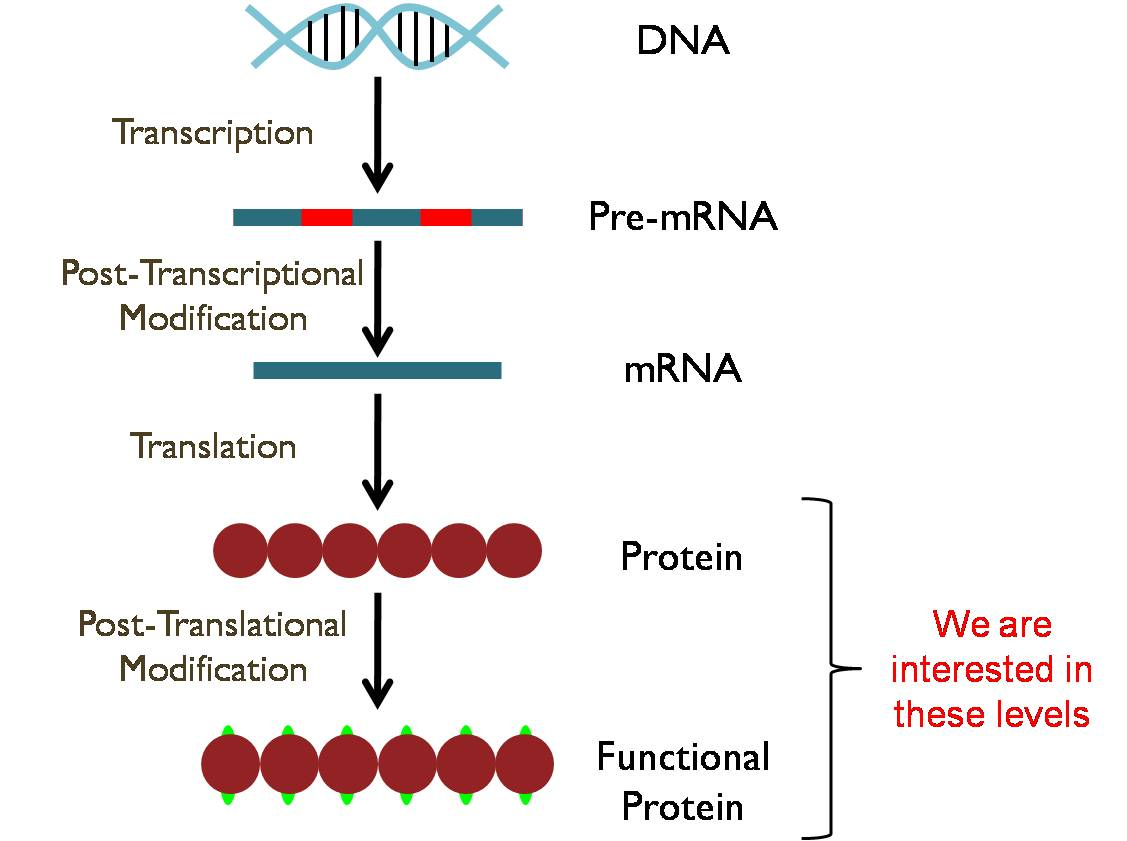
\includegraphics[scale=0.55]{image/processes.jpg}}
\caption{Basic biological processes of producing functional proteins from DNA.}
\label{fig:processes}
\end{figure}

There are many ways to study proteins. For example, physical structures of a protein can be studied by X-ray crystallography~\citep{Blow2002}, protein-protein interactions can be studied using the yeast two-hybrid system~\citep{Fields1989}, and the abundance of an individual protein under a defined condition can be studied using isotopic-labelling. The latter, referred to as \emph{quantitative proteomics}, is achieved via a process of separating a complex protein mixture into smaller subunits to enable high resolution measurements of the constituent components of proteins. The use of  {\bf Mu}lti-dimensional {\bf P}rotein {\bf I}dentification {\bf T}echnology (MudPIT) together with {\bf i}sobaric {\bf T}ags for {\bf R}elative and {\bf A}bsolute {\bf Q}uantitation (iTRAQ$^{\rm TM}$) is just one technology used to measure protein abundance.  

\subsection{Multi-dimensional protein identification technology} \label{subsec:MudPIT}
Multi-dimensional Protein Identification Technology (MudPIT) is a chromatography-based method, which uses a suite of technologies to separate a peptide mixture in order to identify and quantify the constituent proteins in the original sample \citep{Washburn2001}. The process typically involves the separation of the peptide mixture into three orthogonal dimensions. The first separation of peptide species is by their charge, using \emph{strong cation exchange chromatography} (SCX). This is followed by a second separation by hydrophobicity, using \emph{reversed phase liquid chromatography} (RPLC). The third separation is by mass, and is carried out by \emph{mass spectrometry} (MS). The combination of all three separation steps reduces the complexity of the sample and enables high throughput protein analysis. Each MudPIT \emph{run} thus comprises these three steps of separation.

The SCX column contains immobilised negatively charged sulfonic acids that form an ionic interaction with the positively charged peptides. Hence, the charge separation by SCX divides a protein digest (i.e. a mixture of peptides) into many different fractions based on the strength of the charge interaction between the peptides and the sulfonic acids. Different peptide sequences have different affinities for the SCX resin. This allows for complex peptide mixtures to be fractionated by gradually increasing the concentration of a competing salt solution (for binding to the sulfonic acid groups in a gradient) in a step-wise manner. The salt concentration ranges between 10mM to 500mM. Hence, at each interval of salt concentration, a set of peptides is released into the next MudPIT phase. Each of these charge intervals is termed a \emph{salt step}, and increasing the number of salt steps enables the detection of proteins with low abundance. 

The set of peptides from each charge fraction is then separated by RPLC based on hydrophobicity. This is achieved with a separate column that contains silica beads with chains of 18 carbon atoms attached. The peptides are loaded into the column, where they undergo hydrophobic interactions with the carbon chains. An organic solvent is then added to the column in concentrations that increase over time, causing the peptides to emerge or \emph{elute}, with the least hydrophobic peptides eluting first. Eluted peptides are then detected using the mass spectrometer.

The mass analysis is performed by MS, whereby each peptide's \emph{mass-to-charge ratio} (m/z) is measured and then used to calculate its molecular mass. Peptide separation is described in more detail in \cite{Eidhammer2008}. 

\emph{Tandem mass spectrometry} (MS/MS), which consists of two repeated phases of MS, was used for this study. Peptide fragmentation occurs between the two phases of MS, and identification and quantification of the peptides and proteins is thus based on these peptide fragments. MS/MS enables higher specificity in protein identification and enables more accurate quantification.

MudPIT has some limitations. For example, large variation in signal intensity between different MudPIT runs can make inter-sample comparisons of peptide or protein abundance difficult. This limitation has been resolved by iTRAQ$^{\rm TM}$ labelling, which enables the simultaneous analysis of up to eight distinct protein digests within a single MudPIT run. For this thesis, each MudPIT run is referred to as a \emph{run}. 

\subsection{iTRAQ$^{\rm TM}$ for protein quantitation}\label{subsec:iTRAQ}
In 2004, \citeauthor{Ross2004} introduced a peptide labelling technology, namely isobaric Tags for Relative and Absolute Quantitation (iTRAQ$^{\rm TM}$), enabling differential labelling of peptides in different biological samples. In its initial format, iTRAQ$^{\rm TM}$ comprised four isobaric tags, each consisting of a reporter group, a balance group, and a peptide reactive group. The reactive group binds the N-terminus at the start of each peptide, and, for those peptides contain lysine residues (i.e. amino acid), then also on the lysine's side chain. The four reporter groups have m/z values 114, 115, 116 and 117, with corresponding balance group values of 31, 30, 29 and 28. Each of the four tags thus has an identical total m/z value of 145 Da, making them isobaric. This enables identical peptide species, differentially labelled with the four tags, to be indistinguishable with respect to the intact mass of the peptide when selected for MS/MS~\citep{Ross2004}. For MS/MS, the relative abundances are determined using the reporter ion signals at m/z values of 114, 115, 116 and 117 on the \emph{mass spectrum}, i.e.\ the graphical representation of the peptides and peptide fragments based on their m/z values and abundances. Mass spectra are generated for both phases of MS/MS, i.e.\ for the intact peptide during the first cycle, and for the fragmented peptides during the second fragmentation cycle. The four different labels thus allow the simultaneous analysis of four different samples ~\citep{Ross2004}.
 
\begin{figure}[!htb]
\centering{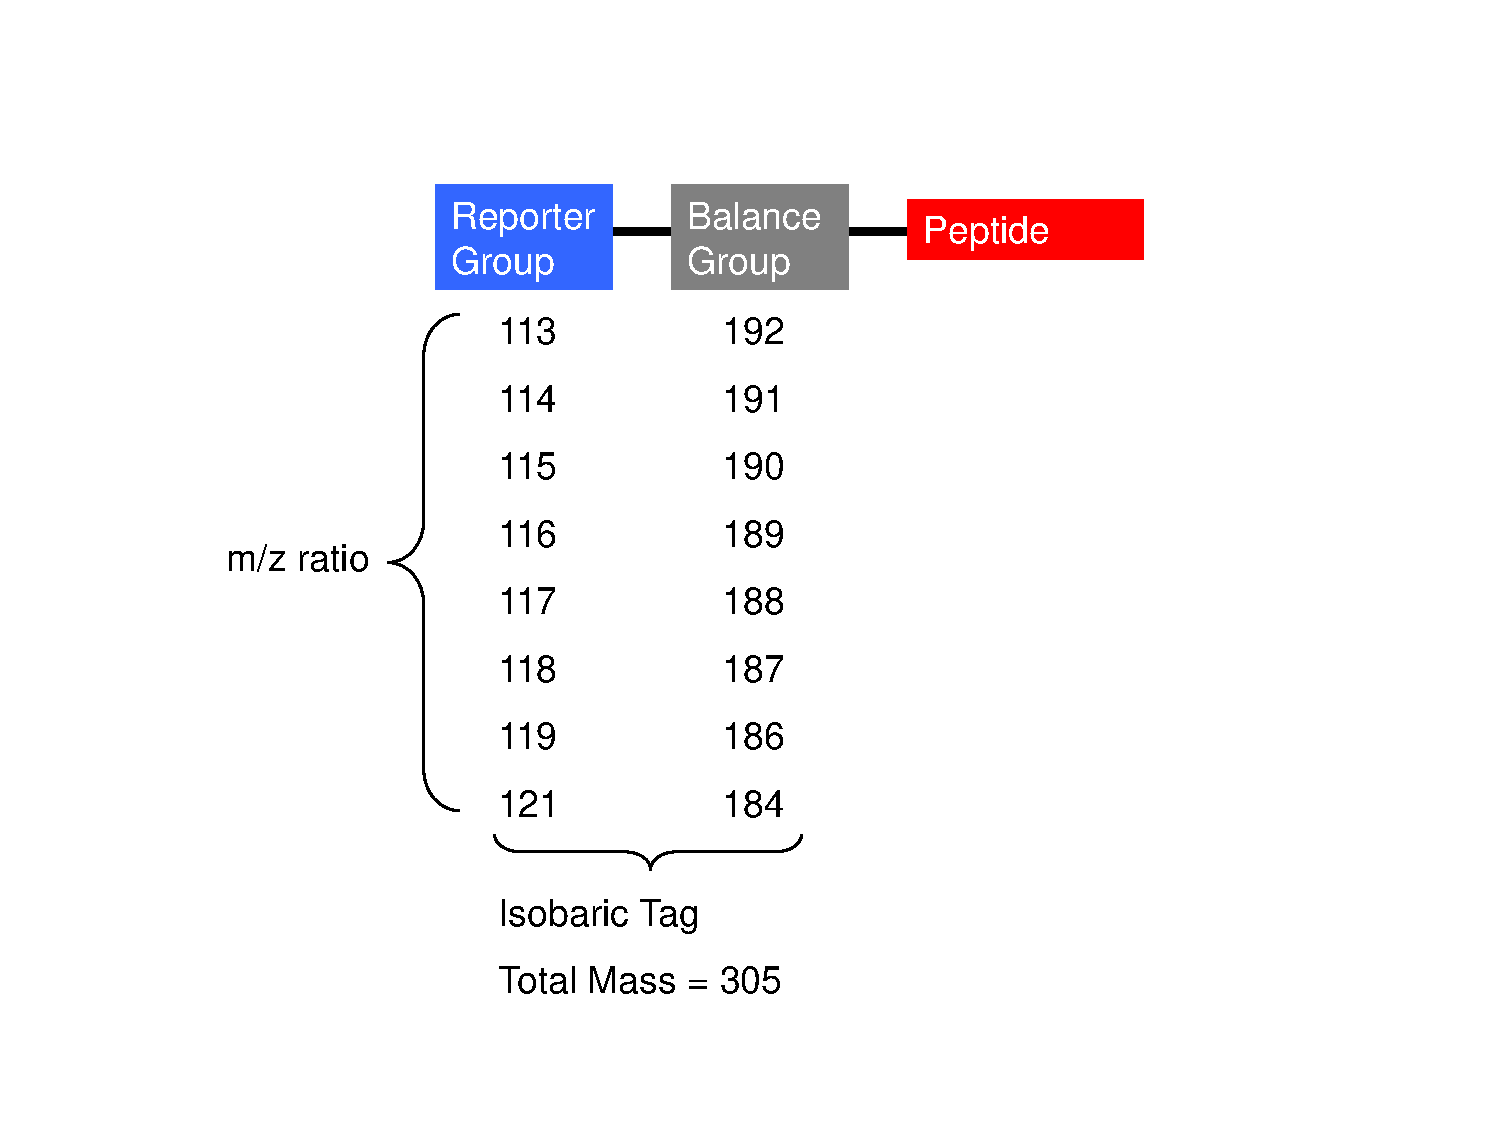
\includegraphics[scale=0.6]{image/iTRAQtags.pdf}}
\caption{Structure of eight-plex-iTRAQ$^{\rm TM}$ tags showing the reporter and balance group masses measured using m/z~\citep{Choe2007}.}
\label{fig:eight-plex}
\end{figure}

\cite{Choe2007} described a new multiplexing strategy, based on the same concept as the four-plex iTRAQ$^{\rm TM}$ system, allowing the simultaneous analysis of up to eight distinct protein samples (see Figure~\ref{fig:eight-plex}). This scheme involves reporter ion signals located at m/z values of 113, 114, 115, 116, 117, 118, 119 and 121. No label is used for an m/z of 120 because it has the same mass as the phenylalanine immonium ion~\citep{Pierce2008}.  For this thesis, each iTRAQ$^{\rm TM}$ tag is referred to as a \emph{tag}. 

\subsection{MudPIT coupled with iTRAQ$^{\rm TM}$: laboratory workflow}\label{sec:MudPITiTRAQ}
Once the target cells or tissues are harvested, each sample is independently processed, including steps for reduction, alkylation, total protein quantification, and enzymatic digestion (usually with trypsin) into many smaller peptide fragments~\citep{Ross2004}. Since proteins exist in a three-dimensional structure, held together by disulfide bonds, reduction breaks down these bonds to produce a two-dimensional linear structure. The alkylation step prevents the reformation of the disulfide bonds. A protein assay is used to measure the total protein content of each sample after reduction and alkylation. This ensures that the total amount of protein to be compared using iTRAQ$^{\rm TM}$ is approximately equal for all samples. Enzymatic digestion with trypsin specifically cleaves the protein immediately after every lysine (K) and arginine (R) residue (see Figure~\ref{fig:protDigest}). 

\begin{figure}[htb]
\centering{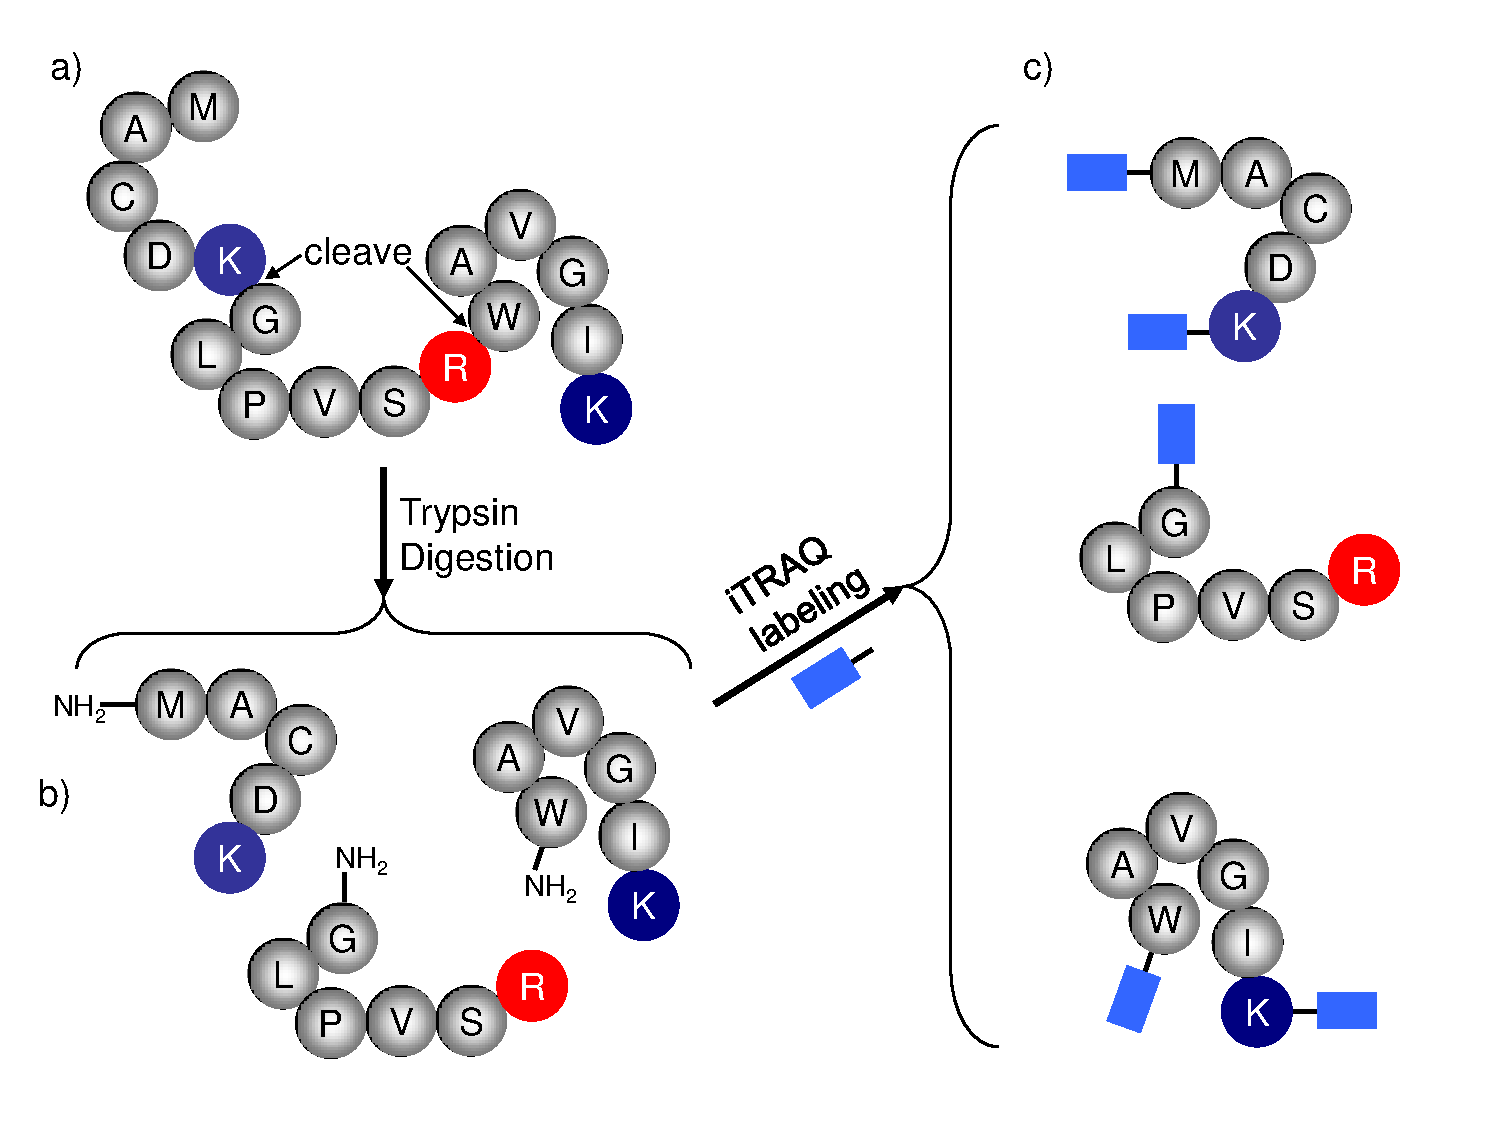
\includegraphics[scale=0.5]{image/proteinDigest.pdf}}
\caption{The process of protein digestion by trypsin. a)Intact protein. b)Digested peptides showing free N-termini. c)Peptides labelled with iTRAQ$^{\rm TM}$ tag.}
\label{fig:protDigest}
\end{figure}

The iTRAQ$^{\rm TM}$ labelling chemistry works by binding the tag to the free N-termini at the start of each peptide and on the K side chain. Thus, with fully efficient enzymatic cleavage, peptides containing one K residue are labelled twice, as the K residue's side-chain also contains a free N-terminus~\citep{Wiese2006}. However, missed cleavages do occur, resulting in some peptides containing more than one K residue. A consequence of this is that these additional K residues are also tagged resulting in a much higher reporter ion abundance due to the additional tags. For example, if a peptide has been labelled twice, the abundance of this peptide is shown as double the true amount in the mass spectrum. To avoid this complication, a \emph{relative quantification} is used instead of an \emph{absolute quantification}. Absolute quantification is calculated as the ratio of a target protein's abundance to a protein of a known concentration either within the same sample, or in a different sample in the same MudPIT run~\citep{Thelen2007}. The sample of known concentration is also referred as a \emph{spike-in}. Relative quantification is the ratio of a particular protein's abundance in one sample to the same protein's abundance in another sample, within the same MudPIT run. Calculating the relative abundance overcomes the issue of the multiple tags on the same peptide because they cancel through this division process. 

Next, approximately equal concentrations of the differentially labelled peptide samples are pooled and undergo the first two phases of MudPIT, i.e. separation by charge with SCX, and separation by hydrophobicity with RPLC (see Section~\ref{subsec:MudPIT}). Finally, the peptide mixture is analysed according to molecular mass using MS/MS. There are many different types of mass spectrometer. An example presented here is the \emph{ElectroSpray Ionisation Quadrupole-Time-Of-Flight tandem mass spectrometer} (ESI-qTOF-MS/MS), called the QSTAR\textsuperscript{\textregistered} (Sciex) (see Figure~\ref{fig:MS/MS}). 
  
\begin{figure}[htb]
\centering{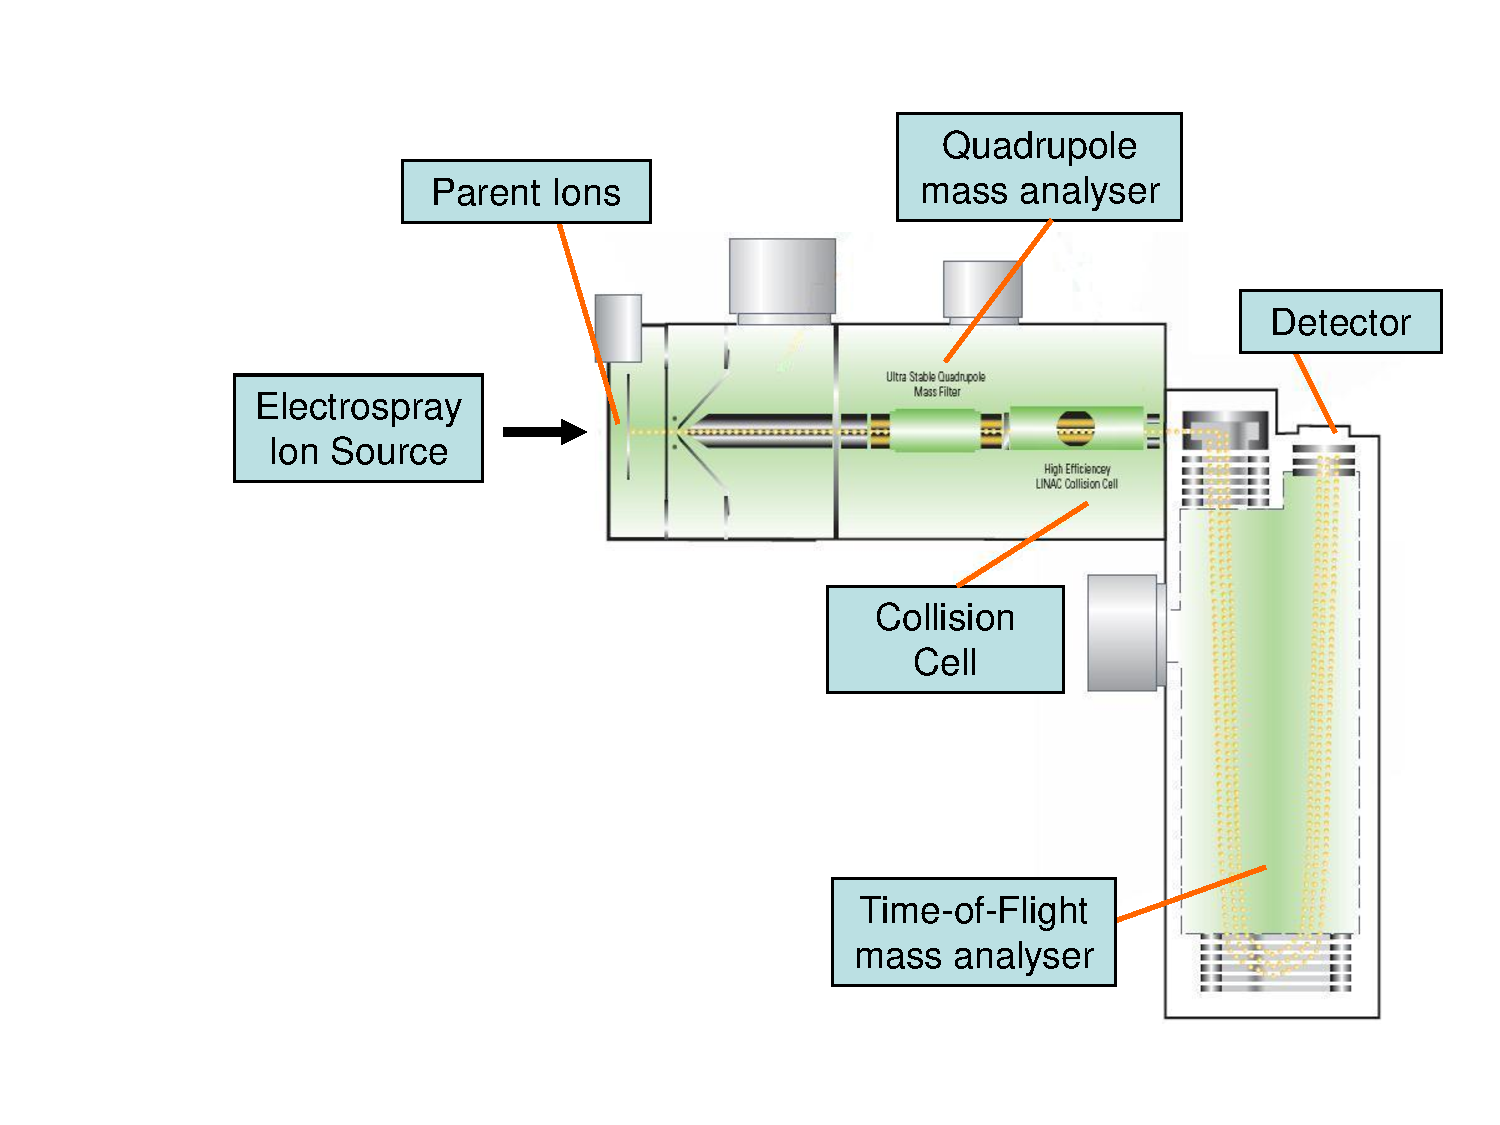
\includegraphics[scale=0.6]{image/qTOF-MSMS.pdf}}
\caption{Schematic of analysis of a protein digest in the QSTAR\textsuperscript{\textregistered} qTOF-MS/MS ~\citep{Applied2004}.}
\label{fig:MS/MS}
\end{figure}

The first step of MS/MS involves subjecting the peptide mixture to ElectroSpray Ionisation (ESI), which transforms each peptide into a positively charged ion, thereby allowing the peptides to be selected, analysed and detected by the mass spectrometer. The separated peptide ions (i.e. ionised peptides) eluting from the RPLC are sprayed continuously into the mass spectrometer for up to 100 minutes for each salt step.   

\begin{figure}[!htb]
\centering{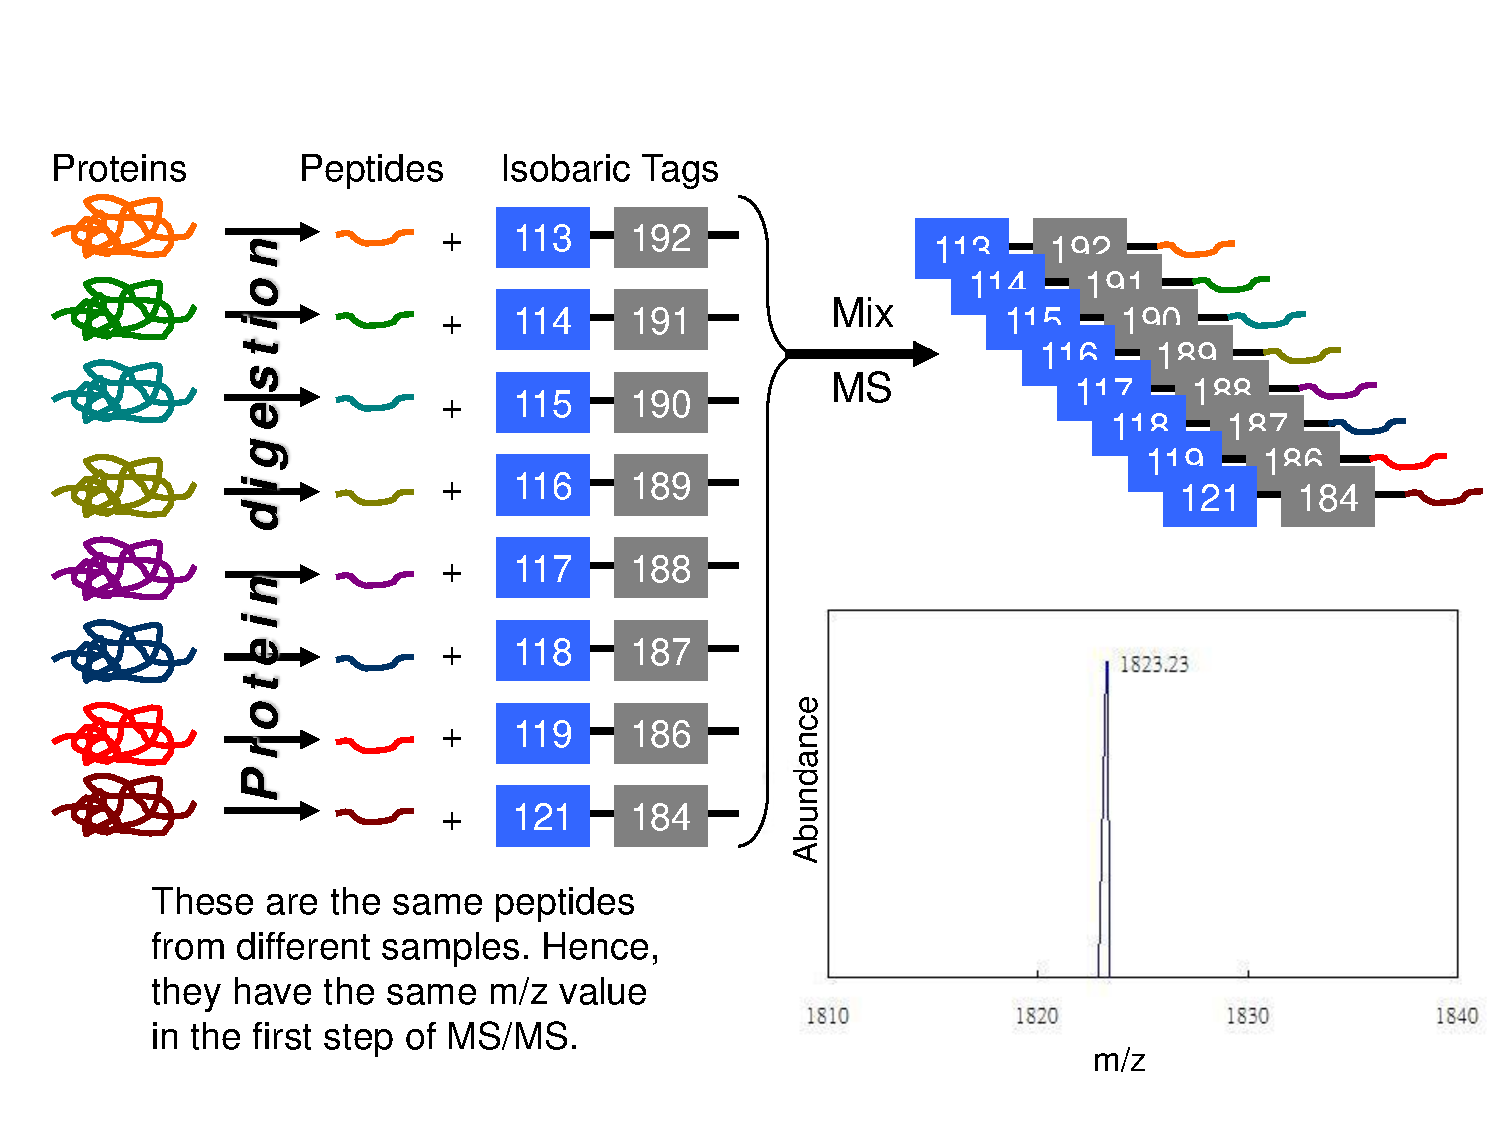
\includegraphics[scale=0.6]{image/MS.pdf}}
\caption{The intensity peak resulting from the mass analysis, of a peptide species with m/z = 1823.23. A single peak is generated for the intact peptide since the mass spectrometer cannot distinguish between the eight samples of origin due to the isobaric tags.}
\label{fig:MS}
\end{figure}

MS/MS consists of two repeated phases of mass analysis and both phases use the Quadrupole-Time-Of-Flight (qTOF) mass analyser. In the first phase, all the peptide ions are passed through the quadrupole mass analyser, and their molecular masses are analysed by the time-of-flight (TOF). The TOF measures the time taken for these ions to travel a known distance. From this, each ion's m/z and abundance is estimated and presented in a MS spectrum (see Figure~\ref{fig:MS}). In the second phase, the peptide ions that have the highest abundance, as detected by the MS, are subsequently isolated by the quadrupole mass analyser. Normally up to three different peptide ions, also known as \emph{precursor} or \emph{parent} ions, are selected in one cycle. Note that these selected peptide ions for the second phase of MS are new peptide ions sprayed by the ESI, as once peptide ions are moved into the TOF they are never recovered. Further, the rate of flow is slow enough that software can instantly inform the quadrupole mass analyser to let a specific peptide pass through. Each of these cycles generally takes around 5.5 seconds: one second to acquire the first MS spectrum, then one, one-and-a-half, and two seconds to acquire the three subsequent MS/MS spectra. Figure~\ref{fig:MSandMSMSspectra} illustrates how the MS and MS/MS spectra are produced under the same time scale, where one MS spectrum will generate the three MS/MS spectra from the three most abundant peptides. 

\begin{figure}[htb]
\centering{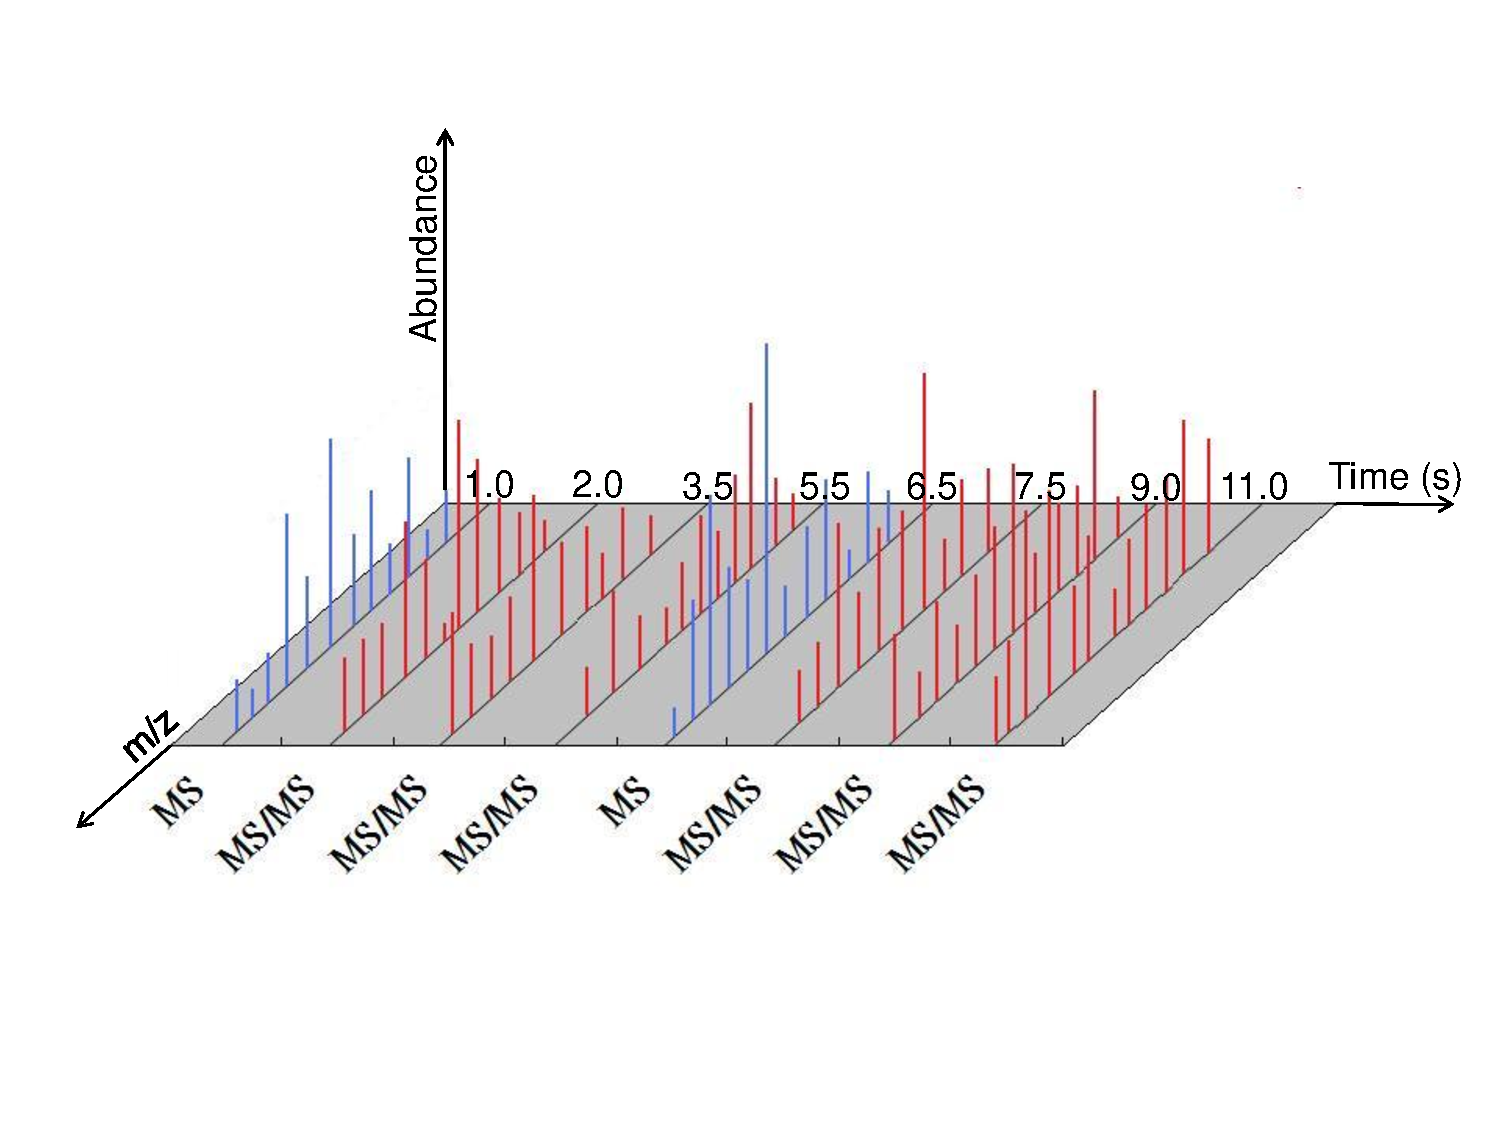
\includegraphics[scale=0.6]{image/MSandMSMSspectra.pdf}}
\caption{Example of MS (blue) and MS/MS (red) spectra.}
\label{fig:MSandMSMSspectra}
\end{figure}

After a specific precursor ion is isolated for the second phase of MS/MS, it moves into a collision cell where it is fragmented into smaller components by collisions with an inert gas. This process, called \emph{collision-induced dissociation} (CID), cleaves the peptide bonds and the chemical bonds with the iTRAQ$^{\rm TM}$ tags. This produces b-ions, y-ions and iTRAQ$^{\rm TM}$ reporter ions (see Figure~\ref{fig:CID}) ~\citep{Ross2004}. The molecular masses of these fragment ions are measured in the TOF. The abundances of the iTRAQ$^{\rm TM}$ labels are estimated from the peaks in the 113 to 121 m/z reporter ion regions. The area under each of these peaks serves as an approximation for the abundance of the peptide in a given sample. The rest of the peaks consist mainly of b- and y- ions, and their m/z are used for peptide identification by comparing the molecular weights of the experimental fragments (i.e. MS and MS/MS spectra) to theoretical fragments generated by in-silico fragmentation of peptides in an appropriate database (see Figure~\ref{fig:spectrum}).

\begin{figure}[!htb]
\centering{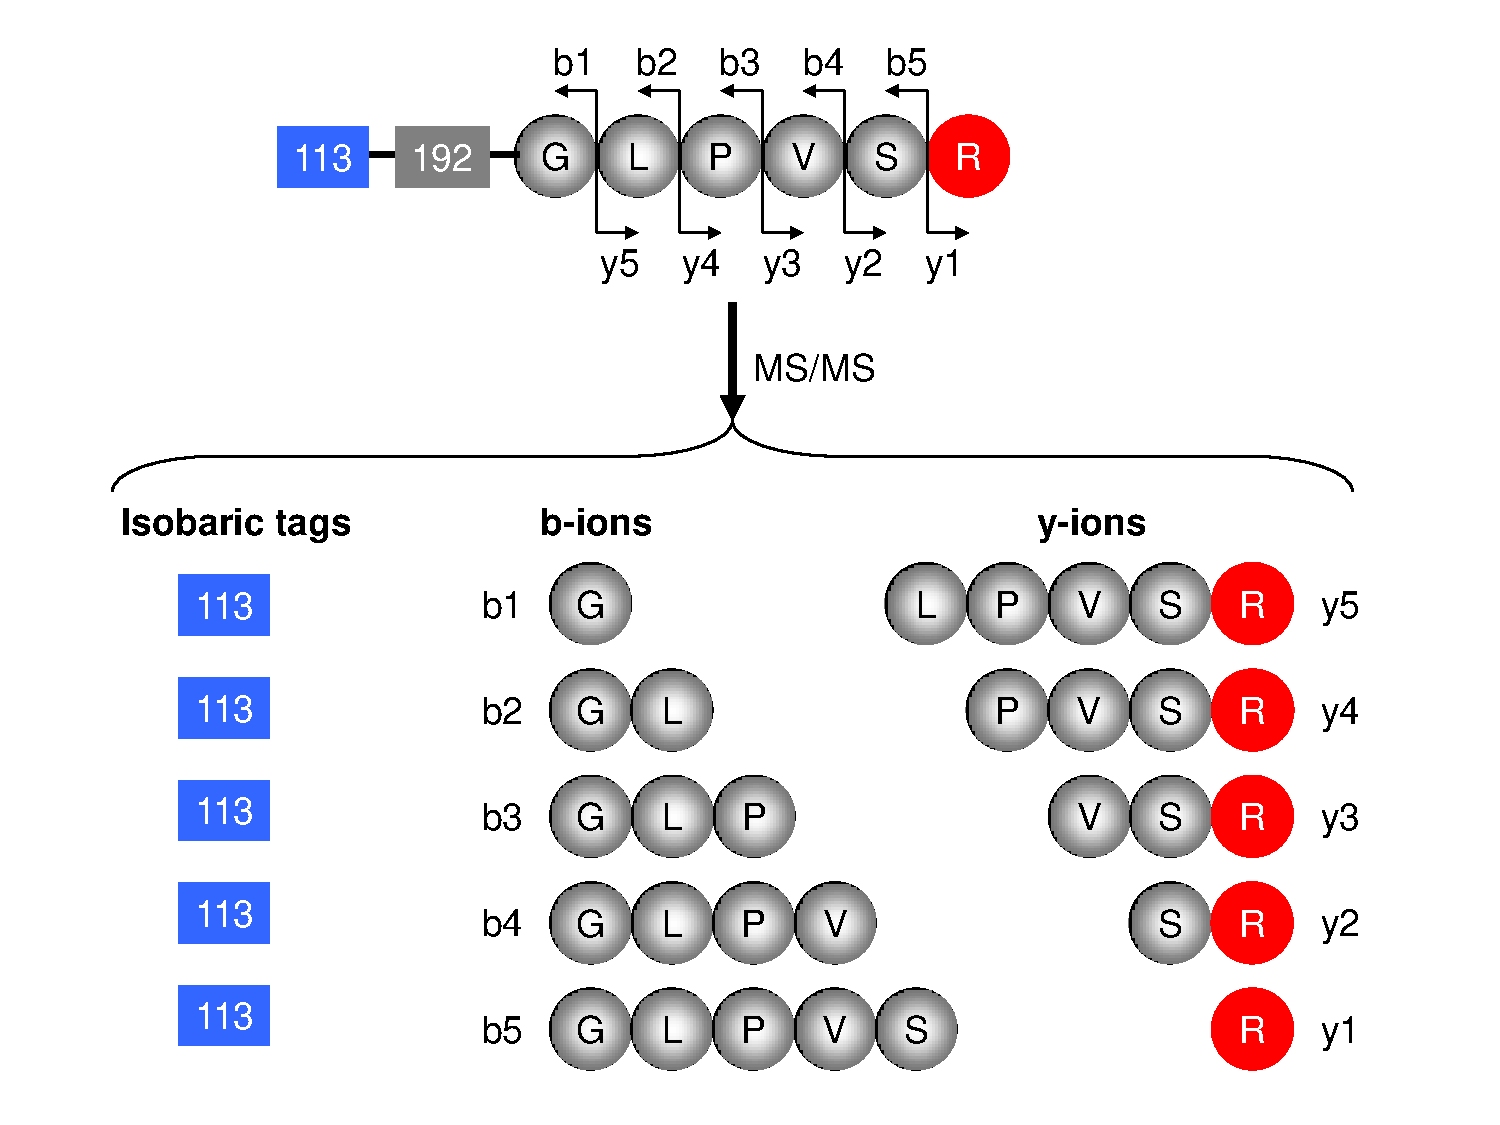
\includegraphics[scale=0.45]{image/CID.pdf}}
\caption{Possible b- and y-ions generated by collision-induced dissociation.}
\label{fig:CID}
\end{figure}

\begin{figure}[!htb]
\centering{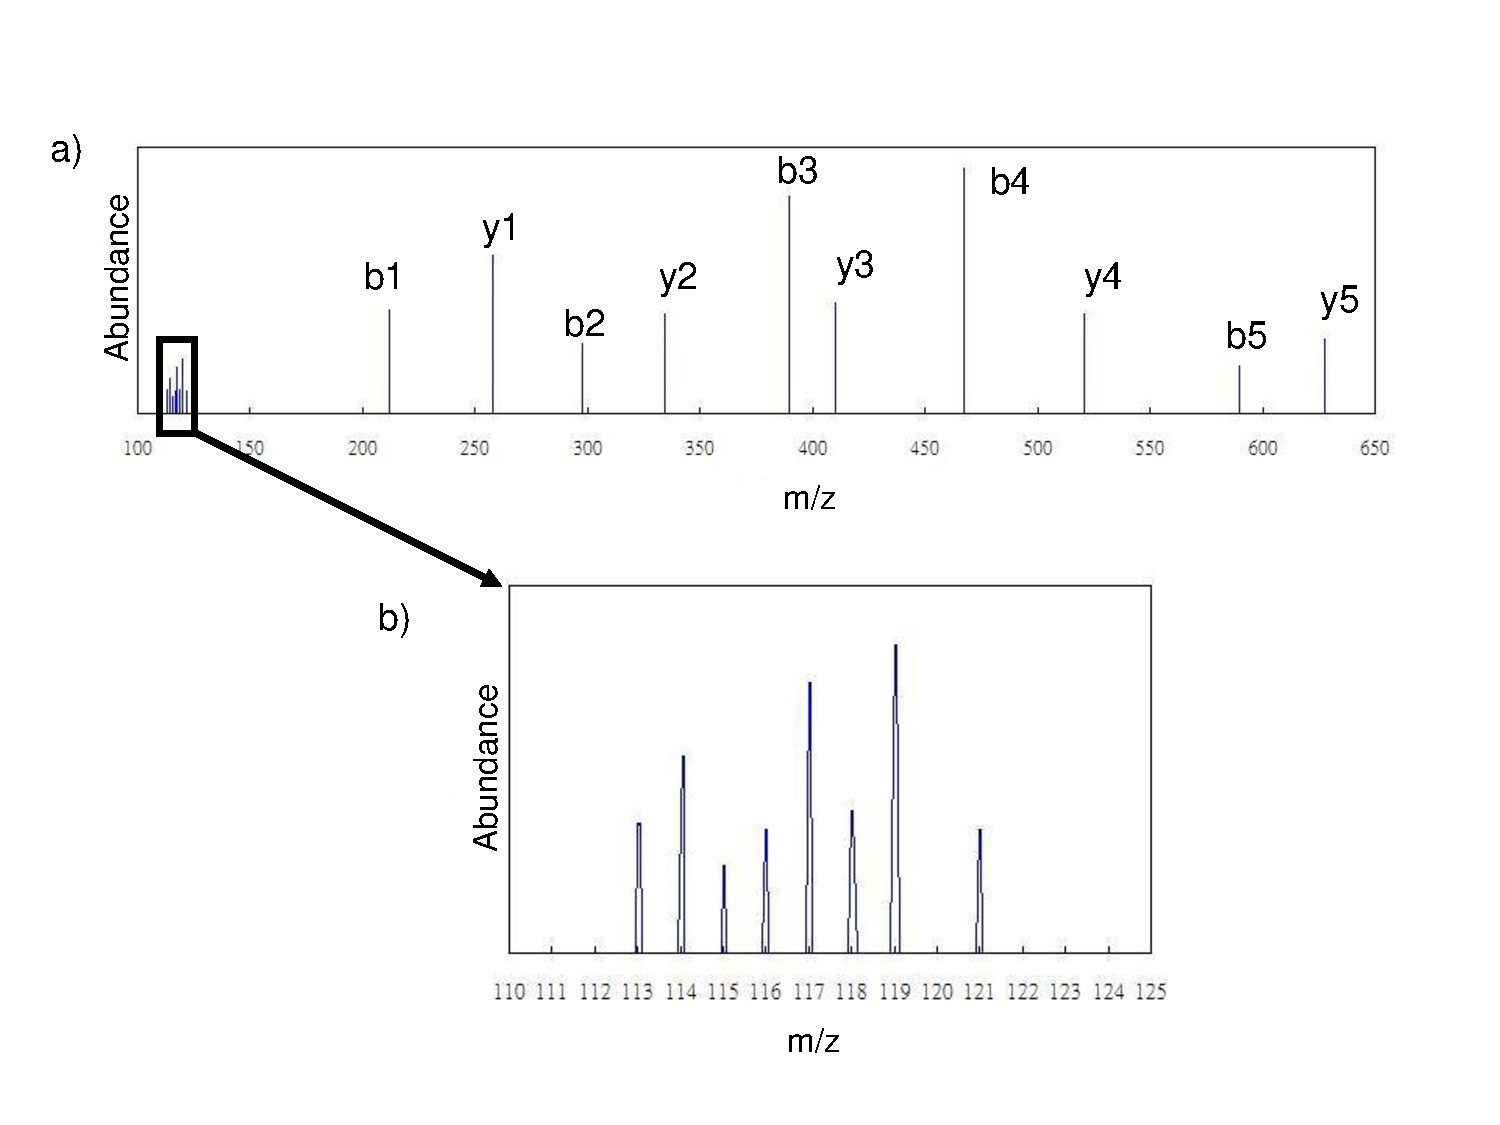
\includegraphics[scale=0.55]{image/mockMSspectra.pdf}}
\caption{a) MS/MS spectra showing the b- and y-ions, and b) zoom-in into 113 to 121 m/z reporter ion region.}
\label{fig:spectrum}
\end{figure}

\subsection{Data generation from MudPIT-iTRAQ$^{\rm TM}$}\label{sec:data}
In every MudPIT run, the QSTAR\textsuperscript{\textregistered} machine generates a WIFF file for each salt step that is performed. Each WIFF file contains all of the MS and MS/MS spectra from the fragmented peptides. There are a number of software packages which are available to perform both peptide-protein identification and the statistical analysis. 

Peptide-to-protein identification involves database searching to identify the proteins that match a given peptide from the MudPIT-iTRAQ$^{\rm TM}$ experimental data. Examples of such software are Mascot$^{\rm TM}$ 2.6 (Matrix Science), SEQUEST\textsuperscript{\textregistered}~\citep{Sadygov2004}, and ProteinPilot$^{\rm TM}$ 5.0 (Sciex). In general, the available software employ a \emph{bottom-up} approach~\citep{Nunn2007}, also known as \emph{shotgun proteomics}~\citep{Nesvizhskii2005}, for protein identification and quantification. The identification method involves a series of peptide matching steps. The mass spectra of the observed fragment ions that were detected in the MudPIT-iTRAQ$^{\rm TM}$ analysis are compared with the mass spectra of theoretical fragment ions, also known as \emph{theoretical spectra}. These theoretical spectra are created from the in-silico tryptic digestion of proteins from an appropriate protein database~\citep{Sadygov2004}. Then, the original intact proteins can be identified from the matched peptides~\citep{Nesvizhskii2005}. 

The database should contain all of the known proteins from a chosen species together with their sequences. Hence, choosing a comprehensive protein sequence database is essential to allow as many peptides as possible to be matched. There are many different protein sequence databases available. The largest and most complete database is Entrez Protein from the National Center for Biotechnology Information (NCBI), because this database is made up of several other databases. However, since this database is generated automatically without any manual correction, some peptide sequences may not be determined correctly. Furthermore, this database has a high degree of sequence redundancy and can slow down the searching process. For a higher quality of sequence annotation, it is more appropriate to use well-curated databases such as Swiss-Prot from the European Bioinformatics Institute (EBI), or Reference Sequence (RefSeq) from NCBI. If the database search cannot find a match for an observed spectrum, then manual peptide sequencing is possible using a process called \emph{de novo peptide sequencing}~\citep{Colinge2007}. Rather than pattern matching the observed spectrum to a theoretical spectrum, de novo peptide sequencing sequences incrementally using the m/z corresponding to the masses of amino acid residues to build the potential sequence of the unknown peptide~\citep{Colinge2007}.

\section{Overview of thesis}
\label{sec:overview}
The primary purpose of this thesis is to develop a method for the computer generation of optimal designs for two-phase multiplex proteomics experiments. This thesis has three parts. The first part, presented in Chapter 2, describes the method of information decomposition of the design in any single- and two-phase experiment, and automates the construction of theoretical ANOVA tables. The second part is the main component of the thesis where we describe a computational approach for finding optimal designs for Phase 2 proteomics experiments. Chapter 3 considers the case of the Phase 1 experiment arranged in a completely randomised design and Chapter 4 considers the case of the Phase 1 experiment arranged in a randomised complete block design (RCBD), or a balanced incomplete block design (BIBD). The third part, presented in Chapter 5, shows how to estimate the variance components and the effective degrees of freedom (EDF) using the restricted maximum likelihood (REML). The comparison of some optimal designs found in Chapters 3 and 4 using the EDF can help clarify the properties of different candidate designs. Chapter 6 summarises and concludes the entire thesis. Furthermore, it presents future directions in the design and analysis of two-phase experiments, in particular, for quantitative high-throughput biotechnology experiments with multiplexing technology. These technologies are currently useful and will remain so for the next decade.


%\bibliographystyle{apalike}
%\bibliography{ref}

%\end{document}
